% Options for packages loaded elsewhere
\PassOptionsToPackage{unicode}{hyperref}
\PassOptionsToPackage{hyphens}{url}
\PassOptionsToPackage{dvipsnames,svgnames,x11names}{xcolor}
%
\documentclass[
]{article}

\usepackage{amsmath,amssymb}
\usepackage{iftex}
\ifPDFTeX
  \usepackage[T1]{fontenc}
  \usepackage[utf8]{inputenc}
  \usepackage{textcomp} % provide euro and other symbols
\else % if luatex or xetex
  \usepackage{unicode-math}
  \defaultfontfeatures{Scale=MatchLowercase}
  \defaultfontfeatures[\rmfamily]{Ligatures=TeX,Scale=1}
\fi
\usepackage{lmodern}
\ifPDFTeX\else  
    % xetex/luatex font selection
    \setmainfont[]{Latin Modern Roman}
  \setmathfont[]{Latin Modern Math}
\fi
% Use upquote if available, for straight quotes in verbatim environments
\IfFileExists{upquote.sty}{\usepackage{upquote}}{}
\IfFileExists{microtype.sty}{% use microtype if available
  \usepackage[]{microtype}
  \UseMicrotypeSet[protrusion]{basicmath} % disable protrusion for tt fonts
}{}
\makeatletter
\@ifundefined{KOMAClassName}{% if non-KOMA class
  \IfFileExists{parskip.sty}{%
    \usepackage{parskip}
  }{% else
    \setlength{\parindent}{0pt}
    \setlength{\parskip}{6pt plus 2pt minus 1pt}}
}{% if KOMA class
  \KOMAoptions{parskip=half}}
\makeatother
\usepackage{xcolor}
\setlength{\emergencystretch}{3em} % prevent overfull lines
\setcounter{secnumdepth}{5}
% Make \paragraph and \subparagraph free-standing
\makeatletter
\ifx\paragraph\undefined\else
  \let\oldparagraph\paragraph
  \renewcommand{\paragraph}{
    \@ifstar
      \xxxParagraphStar
      \xxxParagraphNoStar
  }
  \newcommand{\xxxParagraphStar}[1]{\oldparagraph*{#1}\mbox{}}
  \newcommand{\xxxParagraphNoStar}[1]{\oldparagraph{#1}\mbox{}}
\fi
\ifx\subparagraph\undefined\else
  \let\oldsubparagraph\subparagraph
  \renewcommand{\subparagraph}{
    \@ifstar
      \xxxSubParagraphStar
      \xxxSubParagraphNoStar
  }
  \newcommand{\xxxSubParagraphStar}[1]{\oldsubparagraph*{#1}\mbox{}}
  \newcommand{\xxxSubParagraphNoStar}[1]{\oldsubparagraph{#1}\mbox{}}
\fi
\makeatother


\providecommand{\tightlist}{%
  \setlength{\itemsep}{0pt}\setlength{\parskip}{0pt}}\usepackage{longtable,booktabs,array}
\usepackage{calc} % for calculating minipage widths
% Correct order of tables after \paragraph or \subparagraph
\usepackage{etoolbox}
\makeatletter
\patchcmd\longtable{\par}{\if@noskipsec\mbox{}\fi\par}{}{}
\makeatother
% Allow footnotes in longtable head/foot
\IfFileExists{footnotehyper.sty}{\usepackage{footnotehyper}}{\usepackage{footnote}}
\makesavenoteenv{longtable}
\usepackage{graphicx}
\makeatletter
\def\maxwidth{\ifdim\Gin@nat@width>\linewidth\linewidth\else\Gin@nat@width\fi}
\def\maxheight{\ifdim\Gin@nat@height>\textheight\textheight\else\Gin@nat@height\fi}
\makeatother
% Scale images if necessary, so that they will not overflow the page
% margins by default, and it is still possible to overwrite the defaults
% using explicit options in \includegraphics[width, height, ...]{}
\setkeys{Gin}{width=\maxwidth,height=\maxheight,keepaspectratio}
% Set default figure placement to htbp
\makeatletter
\def\fps@figure{htbp}
\makeatother
% definitions for citeproc citations
\NewDocumentCommand\citeproctext{}{}
\NewDocumentCommand\citeproc{mm}{%
  \begingroup\def\citeproctext{#2}\cite{#1}\endgroup}
\makeatletter
 % allow citations to break across lines
 \let\@cite@ofmt\@firstofone
 % avoid brackets around text for \cite:
 \def\@biblabel#1{}
 \def\@cite#1#2{{#1\if@tempswa , #2\fi}}
\makeatother
\newlength{\cslhangindent}
\setlength{\cslhangindent}{1.5em}
\newlength{\csllabelwidth}
\setlength{\csllabelwidth}{3em}
\newenvironment{CSLReferences}[2] % #1 hanging-indent, #2 entry-spacing
 {\begin{list}{}{%
  \setlength{\itemindent}{0pt}
  \setlength{\leftmargin}{0pt}
  \setlength{\parsep}{0pt}
  % turn on hanging indent if param 1 is 1
  \ifodd #1
   \setlength{\leftmargin}{\cslhangindent}
   \setlength{\itemindent}{-1\cslhangindent}
  \fi
  % set entry spacing
  \setlength{\itemsep}{#2\baselineskip}}}
 {\end{list}}
\usepackage{calc}
\newcommand{\CSLBlock}[1]{\hfill\break\parbox[t]{\linewidth}{\strut\ignorespaces#1\strut}}
\newcommand{\CSLLeftMargin}[1]{\parbox[t]{\csllabelwidth}{\strut#1\strut}}
\newcommand{\CSLRightInline}[1]{\parbox[t]{\linewidth - \csllabelwidth}{\strut#1\strut}}
\newcommand{\CSLIndent}[1]{\hspace{\cslhangindent}#1}

\usepackage{booktabs}
\usepackage{longtable}
\usepackage{array}
\usepackage{multirow}
\usepackage{wrapfig}
\usepackage{float}
\usepackage{colortbl}
\usepackage{pdflscape}
\usepackage{tabu}
\usepackage{threeparttable}
\usepackage{threeparttablex}
\usepackage[normalem]{ulem}
\usepackage{makecell}
\usepackage{xcolor}
\setlength{\defaultaddspace}{0pt}
\usepackage{arxiv}
\usepackage{orcidlink}
\usepackage{amsmath}
\usepackage[T1]{fontenc}
\makeatletter
\@ifpackageloaded{caption}{}{\usepackage{caption}}
\AtBeginDocument{%
\ifdefined\contentsname
  \renewcommand*\contentsname{Table of contents}
\else
  \newcommand\contentsname{Table of contents}
\fi
\ifdefined\listfigurename
  \renewcommand*\listfigurename{List of Figures}
\else
  \newcommand\listfigurename{List of Figures}
\fi
\ifdefined\listtablename
  \renewcommand*\listtablename{List of Tables}
\else
  \newcommand\listtablename{List of Tables}
\fi
\ifdefined\figurename
  \renewcommand*\figurename{Figure}
\else
  \newcommand\figurename{Figure}
\fi
\ifdefined\tablename
  \renewcommand*\tablename{Table}
\else
  \newcommand\tablename{Table}
\fi
}
\@ifpackageloaded{float}{}{\usepackage{float}}
\floatstyle{ruled}
\@ifundefined{c@chapter}{\newfloat{codelisting}{h}{lop}}{\newfloat{codelisting}{h}{lop}[chapter]}
\floatname{codelisting}{Listing}
\newcommand*\listoflistings{\listof{codelisting}{List of Listings}}
\makeatother
\makeatletter
\makeatother
\makeatletter
\@ifpackageloaded{caption}{}{\usepackage{caption}}
\@ifpackageloaded{subcaption}{}{\usepackage{subcaption}}
\makeatother

\ifLuaTeX
  \usepackage{selnolig}  % disable illegal ligatures
\fi
\usepackage{bookmark}

\IfFileExists{xurl.sty}{\usepackage{xurl}}{} % add URL line breaks if available
\urlstyle{same} % disable monospaced font for URLs
\hypersetup{
  pdftitle={POPULATION INDICES, TRENDS, AND DISTRIBUTION OF BREEDING WATERBIRDS ON THE ARCTIC COASTAL PLAIN, ALASKA, 2007-2024},
  pdfauthor={HEATHER M. WILSON, DAVID E. SAFINE, CHARLES J. FROST, AND ERIK E. OSNAS},
  colorlinks=true,
  linkcolor={blue},
  filecolor={Maroon},
  citecolor={Blue},
  urlcolor={Blue},
  pdfcreator={LaTeX via pandoc}}


\newcommand{\runninghead}{A Preprint }
\renewcommand{\runninghead}{Arctic Coastal Plain Aerial Breeding
Population Survey Report 2007-2024 }
\title{POPULATION INDICES, TRENDS, AND DISTRIBUTION OF BREEDING
WATERBIRDS ON THE ARCTIC COASTAL PLAIN, ALASKA, 2007-2024}
\def\asep{\\\\\\ } % default: all authors on same column
\author{\textbf{HEATHER M. WILSON, DAVID E. SAFINE, CHARLES J. FROST,
AND ERIK E. OSNAS}\\Migratory Bird Management\\U.S Fish and Wildlife
Service\\Anchorage, AK 99503\\\href{mailto:heather\_wilson@fws.gov,
david\_safine@fws.gov, charles\_frost@fws.gov, and
erik\_osnas@fws.gov}{heather\_wilson@fws.gov, david\_safine@fws.gov,
charles\_frost@fws.gov, and erik\_osnas@fws.gov}}
\date{}
\begin{document}
\maketitle


\section*{ABSTRACT}\label{abstract}
\addcontentsline{toc}{section}{ABSTRACT}

The Arctic Coastal Plain Aerial Breeding Population Survey (ACP Survey)
provides data on the distribution and relative abundance of 33 bird
species (including 29 waterbird species) that nest in northern Alaska.
Among those reported are species of conservation concern, including
threatened spectacled and Steller's eiders, yellow-billed loons, and
snow geese. This report focuses on results from the 2018-2024 ACP
surveys and presents population indices for all species from 2007- 2024.
No surveys were conducted in 2020-2021 due to the COVID pandemic. For
surveys flown in 2018, 2019, 2022-2024, the respective indicated total
bird indices and their associated 95\% confidence intervals (CI) for
spectacled eiders were 4,745 (3,212 - 6,277), 3,738 (2,820 - 4,656),
2,335 (1,556 - 3,115), 2,284 (1,494 - 3,074), and 2,008 (1,138 - 2,878);
and for Steller's eiders were 95 (0 - 300), 167 (14 - 320), 188 (0 -
468), 96 (0 - 276), 286 (0 - 577). Long-term (2007-2024) mean annual
population indices and trends (and their associated 95\% CIs) for these
species and others of conservation concern, were as follows: spectacled
eiders (indicated total birds) 5,012 (3,661 - 6,362), growth rate 0.93
(0.90 - 0.97); Steller's eiders (indicated total birds) 169 (0 - 466),
growth rate 1.05 (0.75 - 1.44); yellow-billed loons (total birds) 2,120
(1,580 - 2,660), growth rate 1.00 (0.95 - 1.05); and snow geese (total
birds) 41,814 (1,051 - 82,576), growth rate 1.12 (1.00 - 1.25). Our
population indices do not account for incomplete detection or other
sources of bias at this time, although the model we used to estimate
growth rate removes average observer effects. Posterior probabilities
for a long-term (2007--2024) growth rate \textless{} 1.00 were
\textgreater{} 0.975 for scaup, spectacled eiders, king eiders, and
jaeger species, indicating high confidence in long-term population
declines for these species. By the same metrics, posterior probabilities
for population increase were \(\geq\) 0.90 for snow geese and sandhill
cranes, indicating moderate confidence in long-term population increases
for these species, while mallards and common ravens showed moderate
confidence for decreasing trends (\textgreater{} 0.90 posterior
probability of decrease). Growth rates for greater white-fronted geese
and tundra swans indicated relatively stable populations (95\% credible
interval bounds for long-term growth rate were \(\pm\) 3\% of a
long-term growth rate of 1.00), although the posterior probability of a
decrease for tundra swans was 0.91, indicating moderate confidence in a
slow decrease for that species. Confidence in directional trends for all
other species was more limited (\textless{} 0.90 posterior probability
for decrease or \textless{} 0.80 for increase). \newline

\subsection*{\texorpdfstring{\emph{Key
Words}}{Key Words}}\label{key-words}
\addcontentsline{toc}{subsection}{\emph{Key Words}}

Aerial breeding pair survey, Alaska, Arctic Coastal Plain, population
index, growth rate, species occurence, spectacled eider \emph{Somateria
fischeri}, snow goose \emph{Anser caerulescens}, Steller's eider
\emph{Polysticta stelleri}, trend, waterfowl, waterbird, yellow-billed
loon \emph{Gavia adamsii}.

\newpage{}

\section*{INTRODUCTION}\label{introduction}
\addcontentsline{toc}{section}{INTRODUCTION}

The Arctic Coastal Plain (ACP) is a vast area of Arctic lowland tundra
in far northern Alaska important for many species of breeding birds
(Johnson et al. 2007; Bart et al. 2013; Amundson et al. 2019),
especially waterbirds. Importantly, it is the only regularly used
breeding area for the threatened population of Steller's eiders
(\emph{Polysticta stelleri}: USFWS 2002), and one of only three breeding
areas for threatened spectacled eiders (\emph{Somateria fischeri}: USFWS
1996). Additionally, the ACP hosts many other waterbird species of
conservation concern, including red-throated (\emph{Gavia stellata}) and
yellow-billed loons (\emph{G. adamsii}), snow geese (\emph{Anser
caerulescens}), Pacific black brant (\emph{Branta bernicla nigricans}),
common eiders (\emph{S. mollissima}), black (\emph{Melanitta americana})
and white-winged scoters (\emph{Melanitta deglandi}), and long-tailed
ducks (\emph{Clangula hyemalis}).

Annual aerial surveys of waterbirds on the ACP have been conducted since
1986. Prior to 2007, two surveys with different timing and coverage
(i.e., the Original ACP Survey, 1986--2006: Brackney and King 1993;
Mallek, Platte, and Stehn 2007; and the North Slope Eider Survey,
1992--2006: Larned, Stehn, and Platte 2006) were used to monitor
waterbirds on the ACP. In 2007, the two historical surveys were merged
(Stehn, Larned, and Platte 2013), and the amalgamated survey, called the
``Arctic Coastal Plain Aerial Breeding Population Survey'', hereafter
``ACP Survey'' (Larned, Stehn, and Platte 2008, 2012; Stehn, Larned, and
Platte 2013; Stehn 2014; Wilson, Larned, and Swaim 2018) has been flown
annually since 2007 (with the exception of 2020 and 2021, due to the
COVID pandemic). The survey provides distribution and abundance
information for 33 species of birds, including loons, swans, geese,
ducks, gulls, jaegers, terns, and selected landbird species breeding in
northern Alaska. These results provide population status and
distribution information to the Pacific Flyway Council, the Alaska
Migratory Bird Co-Management Council, spectacled and Steller's eider
Recovery Teams, U.S. Fish and Wildlife Service (USFWS), U.S. Geological
Survey, Bureau of Land Management, North Slope Borough, various
non-governmental organizations, local communities, consulting firms, and
industry. This report focuses on the previously unreported 2018-2024
survey data and presents updated population information for all 33 bird
species monitored from 2007-2024.

\begin{figure}

\centering{

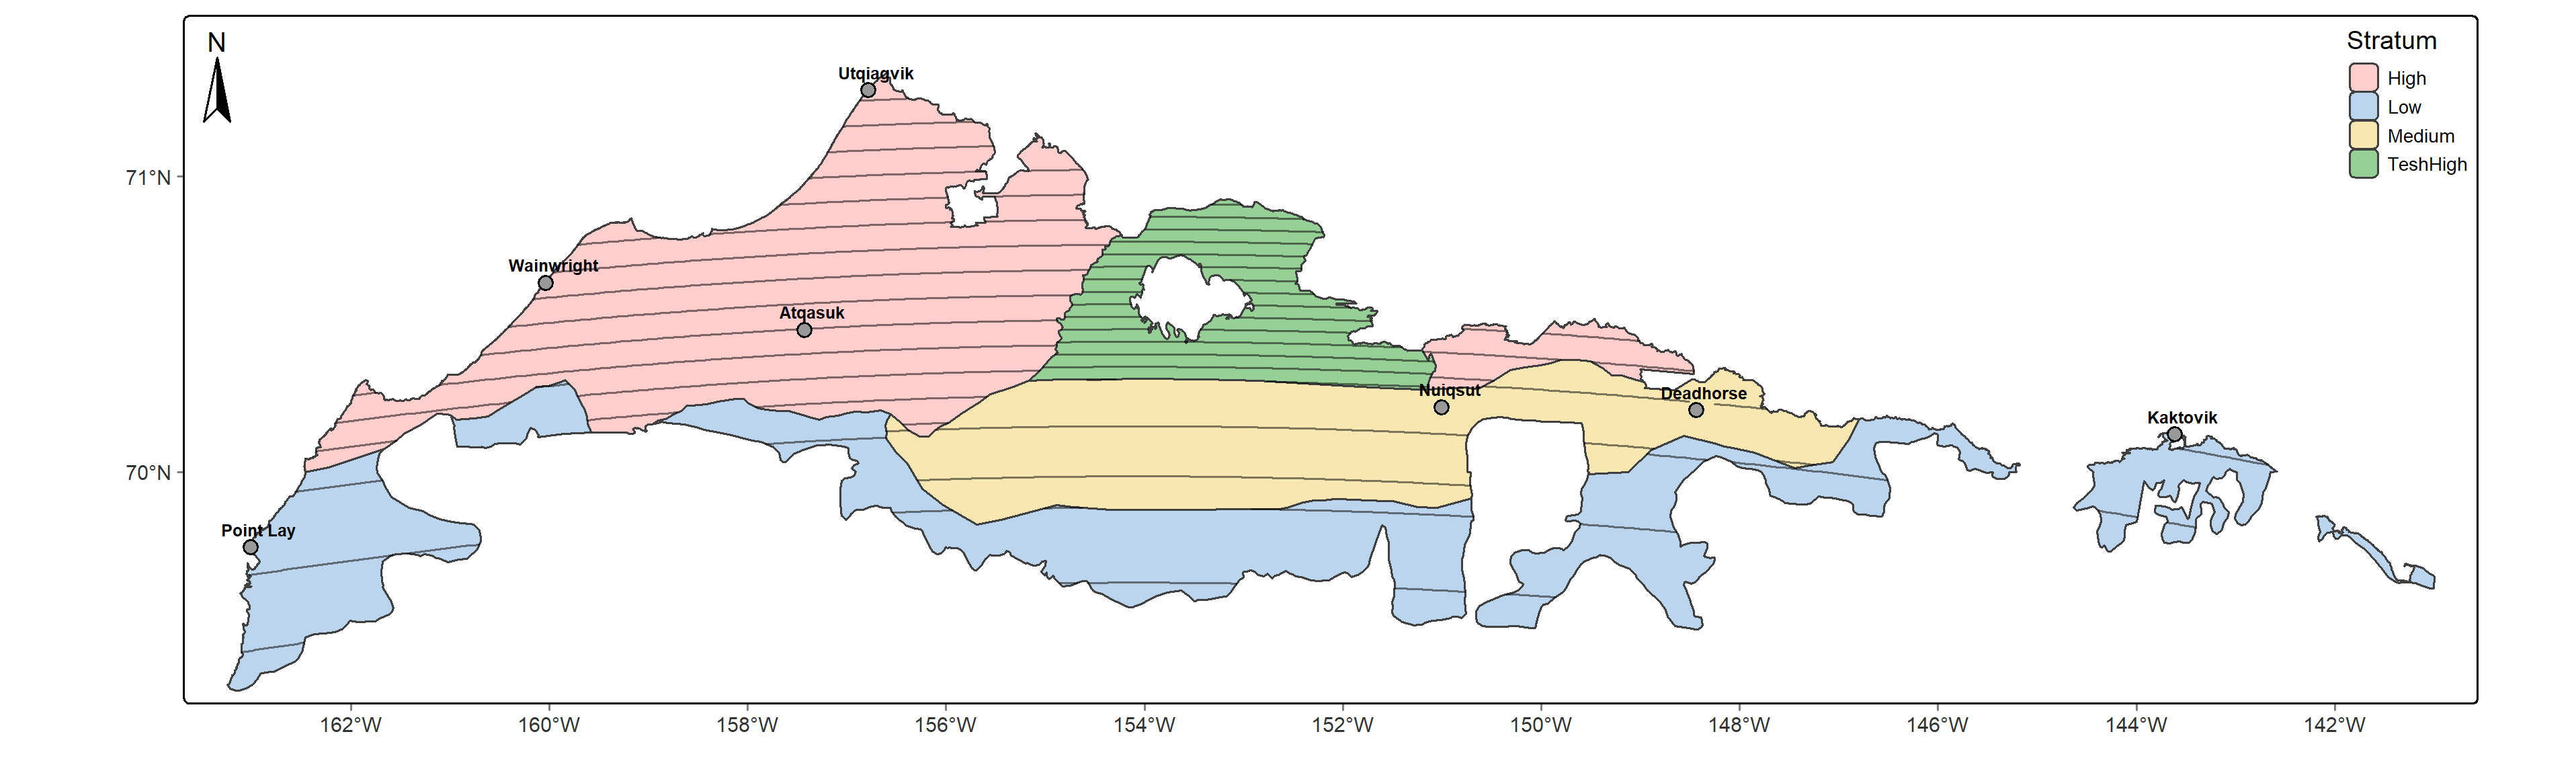
\includegraphics{data/fig1.png}

}

\caption{\label{fig-Fig1}Study area and survey design for the Arctic
Coastal Plain Aerial Breeding Population Survey (ACP Survey) in northern
Alaska, illustrating the 2024 transects, strata, and village locations.
The exact locations of survey transects vary slightly each year based on
a four-year rotating panel within four physiographic and
bird-density-based strata (high, medium, low, and Teshekpuk high).}

\end{figure}%

\section*{METHODS}\label{methods}
\addcontentsline{toc}{section}{METHODS}

\subsection*{Survey Design}\label{survey-design}
\addcontentsline{toc}{subsection}{Survey Design}

The ACP Survey study area encompasses 57,339 \(km^2\), of tundra
wetlands, extending from the Chukchi Sea coast in the west to the
Canadian border in the east, and from the foothills of the Brooks Range
to the Beaufort Sea. As flown since 2007, the ACP Survey is broken into
four physiographic and bird-density-based strata, with a 4-year rotating
panel of systematic strip-transects within each stratum
(Figure~\ref{fig-Fig1}). Herein, the within-strata sampling effort is
proportional to bird densities, such that fewer transects are surveyed
in strata where bird densities are lower. The four-year rotating panel
design results in the panel (i.e., group) of transects being shifted by
25\% of the inter-transect distance each year. The annual inter-transect
distances for each of the four ACP Survey strata are 4.8 km (Teshekpuk
High), 9.6 km (High), 19.2 km (Medium), and 28.8 km {[}Low; Larned,
Stehn, and Platte (2012), Figure~\ref{fig-Fig1}{]}. Given the 400 m
transect width, this results in average annual sampling fractions of
\textasciitilde7.3\%, 3.7\%, 1.8\%, and 1.1\%, in the respective strata.
Thus, within a 4-year panel of transects the inter-transect distances
for each of the four ACP Survey strata become 1.2 km (Teshekpuk High),
2.4 km (High), 4.8 km (Medium), and 7.2 km (Low), resulting in sampling
fractions of \textasciitilde29.1\%, 14.7\%, 7.2\%, and 4.2\%, in the
respective strata over a four-year period. Total areas of each stratum
are Teshekpuk High: 5,654 km\textsuperscript{2}, High: 20,351
km\textsuperscript{2}, Medium: 13,065 km\textsuperscript{2}, and Low:
18,266 km\textsuperscript{2}.

\subsection*{Survey Methods}\label{survey-methods}
\addcontentsline{toc}{subsection}{Survey Methods}

The ACP Survey methodology is based on standard operating procedures for
the North American Waterfowl Breeding Population and Habitat Survey
(USFWS and CWS 1987), with both the left-front seat biologist-pilot and
right-front seat observer recording all waterfowl, loons, gulls,
jaegers, terns, eagles, owls, and ravens seen within a strip transect
encompassing 200 m on either side of the flight path. To estimate the
outer transect boundary, crews determine the required viewing angle
trigonometrically and mark a reference point on the wing strut and side
window for each observer, using a clinometer and marking tape/pens.
Surveys are flown at an approximate ground speed of 161 km/hr
(\textasciitilde87 kts; though actual ground speeds vary due to winds),
and an altitude of 38 m (125 ft) above ground level (AGL), as referenced
by a radar altimeter installed in the aircraft. Georeferenced
observations made from both sides of the aircraft are voice-recorded
into panel-mounted devices for later transcription using the custom
software packages RECORD and TRANSCRIBE (2018-2022: Hodges 2015) and H2
and SCRIBE (2023-present: SWYM 2021). Since 2014, we used a Cessna 206
amphibious-equipped aircraft (Cessna Aircraft Company, Wichita, KS) and
the same survey crew in all of the years for which we are presenting new
data (2018-2019, 2022-2024; Table~\ref{tbl-crew} and
Table~\ref{tbl-results}). The survey required 65, 52, 52, 47, and 47
flight-hours to complete, respectively, in 2018-2019 and 2022-2024, not
including ferry time from Anchorage to and from the study area.

\begingroup\fontsize{10}{12}\selectfont

\begin{longtable}[t]{ccccc}

\caption{\label{tbl-crew}Arctic Coastal Plain Aerial Breeding Population
Survey (ACP Survey) dates and crews (2007-2024). The current ACP Survey
combines the timing of the historical North Slope Eider Survey
(1992-2006) with the geographic coverage of the Original ACP Survey
(1986-2006), and has been flown since 2007. No surveys were flown in
2020 or 2021 due to the COVID pandemic. Aircraft used were either
amphibious-equipped Cessna 206 (C206) or Kodiak 100.}

\tabularnewline

\\
\toprule
\multicolumn{1}{c}{\textbf{ }} & \multicolumn{1}{c}{\textbf{Dates of}} & \multicolumn{1}{c}{\textbf{Pilot}} & \multicolumn{1}{c}{\textbf{Non-pilot}} & \multicolumn{1}{c}{\textbf{ }} \\
\cmidrule(l{3pt}r{3pt}){2-2} \cmidrule(l{3pt}r{3pt}){3-3} \cmidrule(l{3pt}r{3pt}){4-4}
\textbf{Year} & \textbf{Data Collection} & \textbf{Left-front observer} & \textbf{Right-front observer} & \textbf{Aircraft}\\
\midrule
2007 & 14-19 June & W. Larned & R. MacDonald & C206 Amphib\\
2008 & 8-16 June & W. Larned & R. MacDonald & C206 Amphib\\
2009 & 7-15 June & W. Larned & R. MacDonald & C206 Amphib\\
2010 & 11-22 June & W. Larned/K. Bollinger & W. Schock & C206 Amphib\\
2011 & 10-19 June & W. Larned & W. Schock & Kodiak Amphib\\
\addlinespace
2012 & 12-18 June & H. Wilson/ W. Larned & H. Wilson/W. Larned & Kodiak Amphib\\
2013 & 10-17 June & H. Wilson & W. Larned & C206 Amphib\\
2014 & 10-20 June & H. Wilson & W. Larned & C206 Amphib\\
2015 & 8-14 June & H. Wilson & W. Larned & C206 Amphib\\
2016 & 6-13 June & H. Wilson & W. Larned & C206 Amphib\\
\addlinespace
2017 & 11-19 June & H. Wilson & W. Larned & C206 Amphib\\
2018 & 15-25 June & H. Wilson & D. Safine & C206 Amphib\\
2019 & 8 -16 June & H. Wilson & D. Safine & C206 Amphib\\
2020 & No Survey Flown & - & - & -\\
2021 & No Survey Flown & - & - & -\\
\addlinespace
2022 & 14-21 June & H. Wilson & D. Safine & C206 Amphib\\
2023 & 11-18 June & H. Wilson & D. Safine & C206 Amphib\\
2024 & 14-21 June & H. Wilson & D. Safine & C206 Amphib\\
\bottomrule

\end{longtable}

\endgroup{}

\subsection*{Survey Timing and Weather
Conditions}\label{survey-timing-and-weather-conditions}
\addcontentsline{toc}{subsection}{Survey Timing and Weather Conditions}

Timing of survey initiation is intended to coincide with the egg
laying/early incubation period of nesting geese and eiders on the ACP,
and the peak presence of male ducks and pairs of other waterfowl
species. This is a period when nesting habitat is just becoming
available (i.e., ice-free water is visible in most shallow vegetated
wetlands, and tundra vegetation is mostly snow-free around pond
margins), typically within the first three weeks of June. According to
Troy (1997), median nest initiation dates for spectacled eiders at
Prudhoe Bay averaged 15 June from 1982 to 1996, with males departing
within 3--5 days of median initiation. More recent data from Utqiagvik,
estimated average spectacled eider nest initiation to be 14 June (Safine
2013), consistent with indicated average (5-year; 2017-2019, 2021-2022)
nest initiation for cackling geese on the Canning River Delta (14 June;
C. Latty, personal communication, Feb.~11, 2025). Within the first two
weeks of June each year (Table~\ref{tbl-crew}), we refined our survey
start dates based on close monitoring of weather and temperature data,
examining snow and ice-cover changes via satellite
(\href{https://worldview.earthdata.nasa.gov/}{NASA Worldview}) and
web-camera imagery (\url{https://weathercams.faa.gov//}), and by
receiving updates on current landscape conditions from biologists and
other local residents on the ACP. From 2018--2024, weather conditions
varied considerably within and among survey years. Reduced visibility
and ceilings due to coastal fog were the most consistent weather
impediments to surveying in all years of the survey. Fog was
particularly troublesome along the northern coastal fringe of the study
area, where on-shore winds (blowing over the ice), small temperature-dew
point spreads, and daily temperature cycles often created instantaneous,
low-visibility conditions.

\subsection*{Population Indices}\label{population-indices}
\addcontentsline{toc}{subsection}{Population Indices}

We calculated population indices to be consistent with their use in
other USFWS surveys. Duck indices followed the guidance of USFWS and CWS
(1987), and goose, swan, and crane indices followed Eldridge (2003).
Pairs were defined as the total number of male-female pairs (or two
monomorphic birds {[}e.g., geese{]} in close association), not the total
number of birds in pairs (USFWS and CWS 1987). Flocked drakes were
defined as the total number of males observed with one or more other
males and no female present (USFWS and CWS 1987), and were only recorded
for ducks. Flocked drakes in groups of less than 5 birds were doubled
(except for scaup; see below), and flocked drakes in groups of 5 or more
were treated as a flock and not doubled (USFWS and CWS 1987). Flocks
were defined as a closely associated single-sex or mixed-sex grouping of
5 or more birds (or 2 or more birds of different species) that could not
be separated into singles and pairs. For scaup, single drakes and
flocked drakes in groups of less than 5 birds were not doubled as they
were for other ducks. This is because sex ratios in scaup lean heavily
towards males, such that not all males can be assumed to have a female
mate (USFWS and CWS 1987). From 2007 to 2023, our breeding birds index
for scaup did not include flocked drakes in groups of less than 5 birds,
leading to an average bias in the breeding birds index for scaup of
-10\%. Starting in 2024, the breeding birds index for scaup began to
include flocked drakes. Formulas for the calculation of the four
population indices presented in this report are shown below.

For dimorphic species (e.g., ducks {[}except scaup{]}) and some
monomorphic species (cranes and dark geese {[}e.g., greater
white-fronted geese, cackling/Canada geese, and brant{]}):

\begin{center}

\textit{Indicated Breeding Birds = 2(singles + pairs + flocked drakes in groups of < 5 birds)} \newline

\textit{Indicated Total Birds = 2(singles + pairs + flocked drakes in groups of < 5 birds) + birds in flocks} \newline

\end{center}

For the remainder of the monomorphic species (e.g., swans, snow geese, grebes, loons, terns, gulls, jaegers, owls, eagles, ravens) and scaup species:\newline

\begin{center}

\textit{Breeding Birds = singles + 2(pairs) + flocked drakes in groups of < 5 birds} \newline

\textit{Total Birds = singles + 2(pairs) + flocked drakes in groups of < 5 birds + birds in flocks} \newline

\end{center}

\subsection*{The Ratio Estimator}\label{the-ratio-estimator}
\addcontentsline{toc}{subsection}{The Ratio Estimator}

Population totals for each index were calculated using a ratio estimator
(Cochran 1977) with transects as the sample units. The classical ratio
estimator (Cochran 1977) is a straightforward approach that can be used
to estimate the population total of observed birds in a survey area
given a systematic or random sampling design with large sample size
(i.e., number of transects). The ratio estimator is especially good when
the response (i.e., number of birds on a transect) is linearly related
to the length or area of the transect. We employed a stratified
strip-transect design for the majority of our surveys of breeding
waterfowl. Study areas are separated into spatial strata based on
physiographic features and historical bird densities. Strata were
sampled by low-level flights along a series of strip transects, with one
or two observers searching 200 meters out from the transect center.
Observations and sampled areas are then summed across transects within
each stratum to produce strata-specific density estimates. These
densities are then multiplied by associated strata areas to produce
stratum-specific population indices that are summed to produce the
overall population indices,
\[E[\hat Y] = \displaystyle\sum_{i}^{S} \frac{\bar y_i}{\bar a_i} A_i = \displaystyle\sum_{i}^{S} \hat D_i A_i\]
where \(y_i\) are observations and \(a_i\) are sampled areas in strata
\(i\), and \[A_i = \displaystyle\sum_{j}^{M_i} a_{ij}\] with estimated
variance from Williams et al.~(2002), where standard error (SE) is
calculated based on inter-transect variance,~
\[Var(\hat Y) = \displaystyle\sum_{i}^{S} M_i^2 \frac{(1-m_i / M_i)}{m_i} ( s^2_{iy} + \hat {D^2}_i s^2_{ia} - 2 \hat {D_i} s_{iay} ),\]
where \(m_i\) and \(M_i\) are the number of sampled and total transects
in strata \(i\), respectively, and there are \(S\) total strata;~
\[S^2_{ix} = \displaystyle\sum_{j}^{m_i} (x_{ij} - \bar x )/(m_i -1), \]
and~
\[S^2_{ixy} = \displaystyle\sum_{j}^{m_i} (x_{ij} - \bar x )(y_{ij} - \bar y )/(m_i -1).\]
The equations above are observer-specific (i.e., calculated for each
observer independently). However, the estimates presented in this report
are the arithmetic mean of observer-specific estimates (n=2, in most
years). Design transects (Figure~\ref{fig-Fig1}) were used to calculate
survey effort, but flight lines sometimes deviated slightly from the
these due to weather avoidance or other factors. Data manuplulation was
completed using the R (R Core Team 2024) package \texttt{AKaerial}
(Frost 2024).

Population indices presented here do not account for incomplete
detection, though there are efforts to incorporate detection data into
annual population estimates for some species (Wilson, Stehn, and Fischer
2017; Osnas 2024b). Summary statistics were calculated for the indicated
total bird (or total bird) index for each bird species, including the
long-term (2007- 2024) and most recent 3-year averages and their
standard errors (Table~\ref{tbl-results}). Indicated breeding bird (or
breeding bird) indices and indicated total bird (or total bird) indices
for each bird species are presented in the Appendices
(Table~\ref{tbl-SNGO} - Table~\ref{tbl-CORA} and Figure~\ref{fig-SNGO} -
Figure~\ref{fig-CORA}). Throughout, we report point estimates \(\pm\)
(1.96 x SE) as a 95\% confidence interval, except in the simulations for
trends (see next section).

\subsection*{Index Trends}\label{index-trends}
\addcontentsline{toc}{subsection}{Index Trends}

Trajectories in population indices were estimated using generalized
additive models (GAM, Wood 2017) in the R package \texttt{mgcv} (Wood
2021) fit to observer-specific index estimates. The GAM model used a
scaled-t likelihood, a continuous smooth term for year, and a random
effect for observer in the linear predictor. The observer effect allowed
us to remove observer-specific effects from any estimated average
trajectory, and the scaled-t likelihood allowed for extra residual
variance from the trend line over a normal likelihood that might be due
to additional year-specific variance from the trend line. To account for
uncertainty in the index estimate, we used a parametric bootstrap of the
estimated index as the modeled response in the GAM. Thus, for each year,
a response was sampled from a normal distribution (with the mean and
standard deviation of the point estimate), truncated to a small value
(1e-10) for samples \(\leq\) 0, and log-transformed. Then a GAM was fit,
and a sample of the parameters was obtained from a multivariate normal
distribution using the estimated parameter vector and covariance matrix.
Annual predictions over the full time series were made from this
parameter sample after removing the effect of observer, and the results
were saved. This procedure was repeated 300 times. As such, this
procedure is an empricial Bayesian method to approximate the posterior
distribution of the trajectory (Miller 2025). For rarer species, some of
which were not observed in all years (e.g., red-necked grebes and
Steller's eiders), we excluded years when no birds were observed. We did
this because observed zeros in these design-based estimates are more
likely due to non-detection or random sampling, rather than complete
absence of the species in the survey area, and model-fit to data that
included zeros did not produce stable estimates. However, we acknowledge
that this may have resulted in some over-smoothing and bias of estimated
trends for species with zero-count years. For improved methods, that
better account for zero observations in rare species see Osnas (2024b).

\newpage{}

We summarized the simulated yearly GAM predictions (i.e., the posterior
distribution of trajectories) by calculating the mean and standard
deviation for each year. An example of simulated results and
observer-specific estimates for one species (Pacific loon) is shown in
Figure~\ref{fig-loon}. For plots and tables presented in the Results and
Appendices, we do not report the observer-specific index estimates or
individual samples of the smooths, in an effort to reduce clutter.
Instead, we show only the average index between observers in any year,
the mean posterior trajectory, and \(\pm\) 2 standard errors from this
mean.

\begin{figure}

\centering{

\includegraphics[width=0.5\textwidth,height=0.5\textheight]{data/plot_trends/figures/PALO_index_2.png}

}

\caption{\label{fig-loon}An example of the modeled index estimates and
trend results for Pacific loon, accounting for observer effects. Colored
points and bars are observer-specific index estimates, which were
sampled 300 times and used as the response in a generalized additive
model. Individal modeled predictions for each sample are shown by the
thin gray lines. These make up the posterior distribution of modeled
trajectories and are summarized by the orange band (approximate 95\%
credible interval) and the thick gray line (posterior mean). End points
of the modeled predictions (thin gray lines) are used to calculate the
posterior distribution of the long-term growth rate.}

\end{figure}%

We estimated the long-term average growth rate from year \(a\) to \(b\)
for each simulated replicate as

\[T_{b-a} = (\hat N_{b}/\hat N_{a})^{1/(b-a)},\]

where \(\hat N_t\) is the predicted index value at year \(t\) from the
bootstrap replicate GAM model, \(t = a\) is the first year of a non-zero
estimate, and \(t = b\) is the last year. Thus, the growth rate was
calculated as the geometric mean annual change in the model-predicted
index. We summarized growth rate by the mean and 95\% credible interval
across the sampled replicates. We also calculated the posterior
probability of a negative growth rate by summarizing the proportion of
posterior samples that were \textless{} 1 (Pr{[}Trend \textless{} 1{]},
Table~\ref{tbl-results}). We only calculated growth rate for total or
indicated total bird indices shown in Table~\ref{tbl-results}. Code is
available in the file \texttt{plot\_trends\_design.R} at (Osnas 2024a).

\section*{RESULTS}\label{results}
\addcontentsline{toc}{section}{RESULTS}

\subsection*{Survey Timing and Weather
Conditions}\label{survey-timing-and-weather-conditions-1}
\addcontentsline{toc}{subsection}{Survey Timing and Weather Conditions}

Dates of data collection for 2018-2019, and 2022-24 were: 15-25, 8-16,
14-21, 11-18, and 14-21 June, respectively (Table~\ref{tbl-crew}).
Survey timing was the latest on record for the survey in 2018 (15-25
June; Table~\ref{tbl-crew}). The first day of data collection on the ACP
in 2018 was 5 days later than the long-term (2007-2024) average start
date of 10 June. In 2018, in particular, sustained cold temperatures,
strong east winds, and significant snow and ice covered much of the
northern ACP landscape well into June. While 2018, 2022, and 2024 were
on the later end of the range of start dates (Table~\ref{tbl-crew}),
2019 was a relatively early year on the ACP. Breakup chronology on the
ACP varies greatly annually, but in general, we have observed later
breakups in the years we have surveyed since 2017.

\begingroup\fontsize{10}{12}\selectfont

\begin{longtable}[t]{llrrrrcc}

\caption{\label{tbl-results}The most recent 3-year (2022-2024) and
long-term (2007-2024) average population indices and associated standard
errors (SE), as well as long-term annual growth rates (long-term trend),
associated 95\% credible intervals (CI), and posterior probability that
a trend is decreasing (Pr{[}Trend \textless{} 1{]}) for bird species on
the Arctic Coastal Plain Aerial Breeding Population Survey in Alaska.
Index formulas used are species-specific, with indicated total birds
(ITB) used for dimorphic species, dark geese, and sandhill cranes, and
total birds (TB) used for the remaining monomorphic species, other than
dark geese, sandhill cranes, and scaup. See the Methods section for
detailed index definitions and trend calculations. Estimates are not
corrected for incomplete detection, but trends do account for observer
effects.}

\tabularnewline

\\
\toprule
\multicolumn{1}{c}{\textbf{ }} & \multicolumn{1}{c}{\textbf{ }} & \multicolumn{1}{c}{\textbf{3-Year}} & \multicolumn{1}{c}{\textbf{ }} & \multicolumn{1}{c}{\textbf{Long-term}} & \multicolumn{1}{c}{\textbf{ }} & \multicolumn{1}{c}{\textbf{Long-term}} & \multicolumn{1}{c}{\textbf{ }} \\
\cmidrule(l{3pt}r{3pt}){3-3} \cmidrule(l{3pt}r{3pt}){5-5} \cmidrule(l{3pt}r{3pt}){7-7}
\textbf{Species} & \textbf{Index} & \textbf{Average} & \textbf{SE} & \textbf{Average} & \textbf{SE} & \textbf{Trend (CI)} & \textbf{Pr(Trend < 1)}\\
\midrule
Snow goose & TB & 72,025 & 24,401 & 41,814 & 20,797 & 1.12 (1.00 - 1.25) & 0.03\\
Greater white-fronted goose & ITB & 198,988 & 12,014 & 232,847 & 13,604 & 1.00 (0.97 - 1.02) & 0.61\\
Brant & ITB & 15,739 & 4,815 & 14,516 & 3,693 & 1.02 (0.95 - 1.08) & 0.30\\
Cackling/Canada goose & ITB & 14,480 & 2,133 & 13,169 & 2,457 & 1.01 (0.95 - 1.07) & 0.27\\
Tundra swan & TB & 12,881 & 1,377 & 14,833 & 1,388 & 0.99 (0.97 - 1.01) & 0.91\\
\addlinespace
Northern shoveler & ITB & 145 & 110 & 437 & 189 & 0.95 (0.74 - 1.18) & 0.69\\
American wigeon & ITB & 513 & 281 & 724 & 308 & 1.03 (0.89 - 1.16) & 0.36\\
Mallard & ITB & 319 & 109 & 566 & 258 & 0.90 (0.75 - 1.03) & 0.93\\
Northern pintail & ITB & 42,339 & 4,284 & 60,631 & 6,836 & 0.99 (0.95 - 1.03) & 0.73\\
American green-winged teal & ITB & 282 & 112 & 512 & 164 & 0.96 (0.86 - 1.06) & 0.84\\
\addlinespace
Scaup species & TB & 12,295 & 1,258 & 17,557 & 2,366 & 0.95 (0.92 - 0.98) & 1.00\\
Steller's eider & ITB & 191 & 130 & 169 & 152 & 1.05 (0.75 - 1.44) & 0.43\\
Spectacled eider & ITB & 2,210 & 415 & 5,012 & 689 & 0.93 (0.90 - 0.97) & 1.00\\
King eider & ITB & 10,784 & 988 & 17,518 & 1,809 & 0.96 (0.94 - 0.99) & 1.00\\
Common eider & ITB & 699 & 403 & 946 & 827 & 1.02 (0.86 - 1.21) & 0.41\\
\addlinespace
Surf scoter & ITB & 699 & 391 & 262 & 218 & 1.11 (0.68 - 1.62) & 0.28\\
White-winged scoter & ITB & 5,939 & 867 & 9,820 & 3,138 & 1.03 (0.96 - 1.12) & 0.24\\
Black scoter & ITB & 180 & 126 & 361 & 219 & 0.99 (0.69 - 1.45) & 0.59\\
Long-tailed duck & ITB & 32,277 & 1,994 & 43,306 & 2,788 & 0.99 (0.96 - 1.02) & 0.74\\
Red-breasted merganser & ITB & 1,442 & 308 & 1,617 & 311 & 1.01 (0.94 - 1.07) & 0.43\\
\addlinespace
Red-necked grebe & TB & 61 & 60 & 65 & 56 & 0.96 (0.63 - 1.38) & 0.62\\
Sandhill crane & ITB & 709 & 194 & 601 & 224 & 1.06 (0.98 - 1.17) & 0.10\\
Jaeger species & TB & 5,833 & 484 & 8,174 & 602 & 0.96 (0.94 - 0.98) & 1.00\\
Sabine's gull & TB & 12,322 & 1,504 & 13,175 & 1,483 & 1.01 (0.98 - 1.04) & 0.29\\
Glaucous gull & TB & 17,802 & 4,445 & 24,108 & 6,549 & 0.99 (0.96 - 1.02) & 0.78\\
\addlinespace
Arctic tern & TB & 14,403 & 1,393 & 19,395 & 1,799 & 0.98 (0.95 - 1.01) & 0.89\\
Red-throated loon & TB & 3,306 & 396 & 2,625 & 378 & 1.01 (0.97 - 1.05) & 0.34\\
Pacific loon & TB & 22,181 & 1,337 & 29,619 & 1,595 & 0.99 (0.96 - 1.01) & 0.81\\
Yellow-billed loon & TB & 1,682 & 221 & 2,121 & 276 & 1.00 (0.95 - 1.05) & 0.51\\
Golden eagle & TB & 246 & 80 & 262 & 77 & 1.01 (0.92 - 1.10) & 0.43\\
\addlinespace
Short-eared owl & TB & 492 & 89 & 474 & 105 & 1.05 (0.94 - 1.19) & 0.22\\
Snowy owl & TB & 1,140 & 311 & 1,174 & 330 & 0.99 (0.88 - 1.10) & 0.58\\
Common raven & TB & 99 & 48 & 274 & 110 & 0.93 (0.83 - 1.03) & 0.93\\
\bottomrule

\end{longtable}

\endgroup{}

\subsection*{Population Indices}\label{population-indices-1}
\addcontentsline{toc}{subsection}{Population Indices}

We summarize the most recent 3-year average (2022-2024) and long-term
average (2007-2024) population indices, as well as long-term (2007-2024)
posterior mean trajectories (trends) and associated 95\% credible
intervals (CI), as well as posterior probabilities that trends are
decreasing (Pr{[}Trend \textless{} 1{]}) for 33 bird species observed on
the ACP Survey (Table~\ref{tbl-results}). Herein, we follow the
taxonomic ordering of Chesser et al. (2024). For each species, we also
present individual annual population indices (2007-2024) and
trajectories in graphical and tabular formats, and maps of individual
species-observations for 2024 (Appendices: Table~\ref{tbl-SNGO} -
Table~\ref{tbl-CORA} and Figure~\ref{fig-SNGO} - Figure~\ref{fig-CORA}).
Though our maps provide accurate observation locations for each species,
we caution that our location data should not be interpreted as
densities, due to differences in sampling effort across strata
boundaries. Historical density models have been published for our
previous data (Amundson et al. 2019), but more current density-modeling
efforts (see Osnas 2024b) for all species in this report have not yet
been completed.

\section*{DISCUSSION}\label{discussion}
\addcontentsline{toc}{section}{DISCUSSION}

This report describes trends in relative abundance for all common
waterbirds (excluding shorebirds; due to their small size and
inconsistent data collection), owls, eagles, and ravens on the ACP of
Alaska, collected by USFWS from 2007-2024; including 2018--2024 survey
data not previously reported. Upper 95\% credible intervals for
long-term (2007--2024) growth rates of scaup, spectacled eiders, king
eiders, and jaeger species were all \textless{} 1.00 and the posterior
probability that the trend was decreasing was \textgreater{} 0.975,
indicating high confidence in population decreases for those species.
Other species showed less evidence (lower posterior probability) for a
population decrease (Table~\ref{tbl-results}). With less, but still
relatively high confidence, tundra swan (0.91), mallard (0.93), American
green-winged teal (0.84), Arctic tern (0.89), Pacific loon (0.81), and
common raven (0.93) all showed some evidence for a decreasing trend
(Table~\ref{tbl-results}). Snow geese showed a high probability
(\textgreater{} 0.975) of a population increase, with a large magnitude
(up to 25\% per year). Greater white-fronted geese were relatively
stable, with a mean growth rate centered on 1.0 and a 95\% credible
interval bound to less than a 3\% increase or decrease. Growth rate
posterior estimates for northern pintail, long-tailed duck, Sabine's
gull, glaucous gull, and yellow-billed loon showed no strong evidence
for a long-term directional trend, but were instead bound to within 5\%
annual changes from 1.00 and showed large year-specific variation or
increasing and decreasing trends over shorter periods. Posterior
estimates for other species showed less evidence for the sign or
magnitude of long-term population change (Table~\ref{tbl-results}).

Though observer bias is a factor in all aerial surveys, the
experience-level and stability of the ACP Survey crew, particularly the
left-seat pilot-observers, has been remarkably high. From 2007--2024,
there were only two pilot-observers who collected left-seat data (Larned
{[}2007-2011{]} and Wilson {[}2012-2024{]}) and viewed together, seats
occupied by Larned and Wilson represented one third of all data
collected over the duration of the survey (2007-2024;
Table~\ref{tbl-crew}). Given this stability in observer-personnel, the
estimated trends will be unbiased if there is little variation in
detection or other observation processes within observers across years.
We did, however, use a model to statistically remove average observer
effects from the estimated average trajectory. This represents an
improvement over past long-term trend estimates, and lacking any trend
in detection or other observation biases, the trends reported here are
the best currently available for this area without directly estimating
these observer biases. Nevertheless, detection and availability biases
are still largely unaccounted for, affecting our population indices.
Thus, these estimate are not measures of absolute abundance. Though we
do not provide detection-adjusted population estimates for 2007-2024, we
did initiate a study examining observer detection of eiders and other
waterbirds on the ACP in 2015 (Wilson, Stehn, and Fischer 2017) and hope
to incorporate detection and observer-adjusted estimates into future
reports using methods similar to Osnas (2024b).

The trajectories estimated here represent continuous smooth functions
after removing average observer effects. We did not fit other models
that allowed for more complex or discontinuous trends, such as
year-specific random effects or spatially explicit predictions (e.g.
Smith and Edwards 2021; Osnas 2024b). Because many species do show large
year-specific deviations from an average trend, a model with such
effects is likely a better description for these species. Such models
are not well-estimated when fit to the design-based estimates used here.
The model we have used, however, can be viewed as a flexible way to
estimate the average trajectory through time, smoothing over
year-specific variations. Compared to a simple log-linear regression on
point estimates, the current approach provides for more flexible
functional forms of the trajectory, allowing for the identification of
cycles or periods of change. One should keep these points in mind when
interpreting results, as for many species, the year-specific variations
are much larger than the average change over time (e.g., northern
pintail) or show cyclical patterns over a shorter time (e.g.,
long-tailed duck, yellow-billed loon).

Trajectories for rare species (those with observed zero estimates)
should be interpreted with care. We attempted to fit our model by
including zero estimates (after adding a small number and log
transforming) but the GAM often failed to find stable estimates, so we
used only positive estimates. This will have two important consequences.
First, trajectories may be biased if there is a trend in the frequency
of zero observations in the time series. Second, the GAM will tend to
produce smoother trajectories than if the zeros were included. For
example, the Steller's eider trajectory is essential a flat line
(Figure~\ref{fig-STEI}); whereas Osnas (2024b) found clear cyclical
patterns in the trajectory when a different GAM model was fit to
smaller-scale, spatially-explicit counts that included zero-counts.
Interestingly, Amundson et al. (2019) also excluded zero-counts in a
spatially-explicit GAM, and found a flat trajectory for Steller's eider
over a much longer time period; suggesting that the smooth GAM is due to
a reduction in data when most observations are excluded. We expect
similar patterns for other rare species. However, for more common
species that do not include zero estimates, we believe the current model
should approximate temporal trajectories in relative abundance. In the
future, we also hope to fit a spatial model to the full set of species.

Although the long-standing, continental-scale aerial Waterfowl Breeding
Population and Habitat Survey (WBPHS) samples most of Alaska's primary
waterfowl production areas, it has never included the rich wetlands of
the Arctic Coastal Plain of Alaska or the high-Arctic of Canada in its
annual efforts. Further, while several targeted monitoring programs for
specific species or limited areas of the ACP have been conducted; to our
knowledge, the ACP Survey represents the most comprehensive aerial
survey of Arctic-breeding waterbirds in existence. The analysis and
implementation of a multi-species, aerial monitoring program such as the
ACP Survey is challenging due to the inherent variability of the natural
ecosystem, the varied natural histories of 30+ species, and the
logistical difficulties of conducting aerial surveys in the Arctic.
Moreover, it is difficult to achieve adequate within-year sampling of
such a large spatial area within a short annual phenological window.
Surveys of this type are further complicated by several waterfowl
species that exist in extremely low densities and/or breed irregularly
(such as Steller's eiders), making precise estimates and trends
difficult to achieve (though see Osnas 2024b). Collection of such a
long-term data set has been made possible by integrating improvements in
sample design along the way. The sample design used in this survey was
originally developed in 1986 to target breeding ducks (Original ACP
Survey 1986-2006: Mallek, Platte, and Stehn 2007), and later augmented
to better include coastal areas and earlier-nesting species, such as
eiders (North Slope Eider Survey 1992--2006: Larned, Stehn, and Platte
2008). The current redesigned survey (2007--present: Stehn, Larned, and
Platte 2013; Wilson, Larned, and Swaim 2018) amalgamated these two
designs and provides good temporal, spatial, and inferential compromise.
However, the changing distributions and abundances of many waterfowl
species, as well as the rapid and wide-spread landscape changes in the
Arctic, may warrant reevaluation of the current stratification and
overall survey design. Nonetheless, this survey represents one of few
broad-scale, long-term, systematic monitoring efforts for waterbirds in
the Arctic of North America, and perhaps, the world.

\subsection*{\texorpdfstring{\emph{Supplemental
Material}}{Supplemental Material}}\label{supplemental-material}
\addcontentsline{toc}{subsection}{\emph{Supplemental Material}}

Species-specific population indices, trends, and spatial distributions
of observations can be found in the tables and figures of the
Appendices. Original data for the ACP Survey can be found at Science
Base - Alaska Arctic Coastal Plain Breeding Waterbird Aerial Survey
2007-Present \url{https://doi.org/10.7944/f6jd-2985} and point-estimates
(and documentation of their calculation) were sourced from the R package
AKaerial at \url{https://github.com/USFWS/AKaerial}. R Quarto code used
to produce this report, the report itself, and associated tabular data,
can be found at \url{https://doi.org/10.7944/dqf4-2z27}.

\subsection*{\texorpdfstring{\emph{Suggested
Citation}}{Suggested Citation}}\label{suggested-citation}
\addcontentsline{toc}{subsection}{\emph{Suggested Citation}}

Wilson, H.M., Safine, D.E., Frost, C.J., and E.E. Osnas. 2025.
Population indices, trends, and distribution of breeding waterbird on
the Arctic Coastal Plain, Alaska, 2007-2024. Anchorage, Alaska: U.S.
Fish and Wildlife Service, Migratory Bird Management.
\url{https://doi.org/10.7944/dqf4-2z27}

\section*{ACKNOWLEDGEMENTS}\label{acknowledgements}
\addcontentsline{toc}{section}{ACKNOWLEDGEMENTS}

This survey would not be possible without the generous support of the
Bureau of Land Management, with particular thanks to Debora Nigro. We
also extend thanks to Bill Larned for his many years flying and
mentoring on the survey, Michael Swaim for assistance with aviation
survey and hazard maps, and Julian Fischer for his thoughtful report
reviews, project support, and program leadership. We are grateful to the
people of Atqasuk, Alaska for hosting us in their community for so many
years, and for helping with logistics and housing. Finally, we
acknowledge the tremendous contribution of the observers and pilots who
collected aerial waterbird data on the ACP beginning in 1986 (Mallek,
Platte, and Stehn 2007; Stehn, Larned, and Platte 2013), and from 2007
forward (Table~\ref{tbl-crew}), and all those who supported their
efforts.

\begin{figure}[H]

{\centering \includegraphics{data/Crew_picture_Wilson_Safine_ACP_2018_2024.jpg}

}

\caption{Arctic Coastal Plain Aerial Breeding Population Survey Crew
2018-2024: David Safine (right-front seat observer) and Heather Wilson
(left-front seat observer/pilot)}

\end{figure}%

\section*{LITERATURE CITED}\label{literature-cited}
\addcontentsline{toc}{section}{LITERATURE CITED}

\phantomsection\label{refs}
\begin{CSLReferences}{1}{0}
\bibitem[\citeproctext]{ref-Amundson2019}
Amundson, C. L., P. L Flint, R. A. Stehn, R. M. Platte, H. M. Wilson, W.
W. Larned, and J. B. Fischer. 2019. {``Spatio-Temporal Population Change
of Arctic-Breeding Waterbirds on the Arctic Coastal Plain of Alaska.''}
\emph{Avian Conservation and Ecology} 14(1): 18.
\url{https://doi.org/10.5751/ACE-01383140118}.

\bibitem[\citeproctext]{ref-Bart2013}
Bart, J. R., R. M. Platte, B. Andres, S. Brown, J. A. Johnson, and W. W.
Larned. 2013. {``Importance of the National Petroleum Reserve-Alaska for
Aquatic Birds.''} \emph{Conservation Biology} 27: 1304--12.

\bibitem[\citeproctext]{ref-Brackney1993}
Brackney, A. W., and R. J. King. 1993. {``Aerial Breeding Pair Surveys
of the Arctic Coastal Plain of Alaska, 1992.''} Fairbanks, Alaska:
USFWS, Migratory Bird Management.
\url{https://www.arlis.org/docs/vol1/FWS/A/213375107/609888633-1993.pdf}.

\bibitem[\citeproctext]{ref-Chesser2024}
Chesser, R Terry, Shawn M Billerman, Kevin J Burns, Carla Cicero, Jon L
Dunn, Blanca E Hernandez-Banos, Rosa Alicia Jimenez, et al. 2024.
{``Sixty-Fifth Supplement to the American Ornithological Society's
Check-List of North American Birds.''} \emph{Ornithology} 141(3).
\url{https://doi.org/10.1093/ornithology/ukae019}.

\bibitem[\citeproctext]{ref-Cochran1977}
Cochran, W. G. 1977. \emph{Sampling Techniques}. New York, New York:
John Wiley \& Sons.

\bibitem[\citeproctext]{ref-Eldridge2003}
Eldridge, W. D. 2003. {``Population Indices, Trends and Distribution of
Geese, Swans and Cranes on the Yukon-Kuskokwim Delta from Aerial
Surveys, 1985-2002.''} Anchorage, Alaska: USFWS, Migratory Bird
Management.
\url{https://www.arlis.org/docs/vol1/FWS/2003/1493344038.pdf}.

\bibitem[\citeproctext]{ref-r-akaerial}
Frost, Charles. 2024. {``AKaerial: Analysis of Alaska Region Aerial
Survey Data.''} \url{https://github.com/USFWS/AKaerial}.

\bibitem[\citeproctext]{ref-Hodges2015Record}
Hodges, J. I. 2015. {``\href{}{RECORD/TRANSCRIBE Custom Software,
Version 10.2}.''}

\bibitem[\citeproctext]{ref-Johnson2007}
Johnson, J. A., R. B. Lanctot, B. A. Andres, J. R. Bart, S. C. Brown, S.
J. Kendall, and D. C. Payer. 2007. {``Distribution of Breeding
Shorebirds on the Arctic Coastal Plain of Alaska.''} \emph{Arctic} 60:
277--93.

\bibitem[\citeproctext]{ref-Larned2006}
Larned, W. W., R. A. Stehn, and R. M. Platte. 2006. {``Eider Breeding
Population Survey, Arctic Coastal Plain, Alaska, 2006.''} Anchorage,
Alaska: USFWS, Migratory Bird Management.
\url{https://www.arlis.org/docs/vol1/FWS/A/213375107/609897140-2006.pdf}.

\bibitem[\citeproctext]{ref-Larned2008}
---------. 2008. {``Eider Breeding Population Survey, Arctic Coastal
Plain, Alaska, 2007.''} Anchorage, Alaska: USFWS, Migratory Bird
Management.
\url{https://www.arlis.org/docs/vol1/FWS/A/213375107/213375107-2007.pdf}.

\bibitem[\citeproctext]{ref-Larned2012}
---------. 2012. {``Waterfowl Breeding Population Survey, Arctic Coastal
Plain, Alaska, 2011.''} Anchorage, Alaska: USFWS, Migratory Bird
Management.
\url{https://www.north-slope.org/wp-content/uploads/2022/04/acp2011rpt.pdf}.

\bibitem[\citeproctext]{ref-Mallek2007}
Mallek, E. J., R. M. Platte, and R. A. Stehn. 2007. {``Aerial Breeding
Pair Surveys of the Arctic Coastal Plain of Alaska -- 2006.''}
Fairbanks, Alaska: USFWS, Migratory Bird Management.
\url{https://www.arlis.org/docs/vol1/FWS/A/213375107/609888633-2006.pdf}.

\bibitem[\citeproctext]{ref-miller2025bayesian}
Miller, David L. 2025. {``Bayesian Views of Generalized Additive
Modelling.''} \emph{Methods in Ecology and Evolution}.
https://doi.org/\url{https://doi.org/10.1111/2041-210X.14498}.

\bibitem[\citeproctext]{ref-osnasgithub}
Osnas, E. E. 2024a. {``ACP-Mapping.''}
\url{https://github.com/USFWS/ACP-Mapping}.

\bibitem[\citeproctext]{ref-Osnas2024}
---------. 2024b. {``Steller's Eider Population and Density Estimates
from the Arctic Coastal Plain and Utqiagvik Triangle Surveys Using
Generalized Additive Models.''} Anchorage, Alaska: USFWS, Migratory Bird
Management. \url{https://doi.org/10.7944/3vzp-0r93}.

\bibitem[\citeproctext]{ref-R}
R Core Team. 2024. \emph{R: A Language and Environment for Statistical
Computing}. Vienna, Austria: R Foundation for Statistical Computing.
\url{https://www.R-project.org/}.

\bibitem[\citeproctext]{ref-Safine2013}
Safine, D. E. 2013. {``Breeding Ecology of Steller's and Spectacled
Eiders Nesting Near Barrow, Alaska, 2012.''} Fairbanks, Alaska: USFWS,
Ecological Services.
\url{https://www.north-slope.org/wp-content/uploads/2022/04/Barrow_Report_2012_final.pdf}.

\bibitem[\citeproctext]{ref-smith2021north}
Smith, Adam C, and Brandon PM Edwards. 2021. {``North American Breeding
Bird Survey Status and Trend Estimates to Inform a Wide Range of
Conservation Needs, Using a Flexible Bayesian Hierarchical Generalized
Additive Model.''} \emph{The Condor} 123 (1): duaa065.

\bibitem[\citeproctext]{ref-Stehn2014}
Stehn, R. A. 2014. {``Analysis of Aerial Survey Indices Monitoring
Waterbird Populations of the Arctic Coastal Plain, Alaska, 1986-2013.''}
Anchorage, Alaska: USFWS, Migratory Bird Management.
\url{https://www.arlis.org/docs/vol1/FWS/2014/1493362935.pdf}.

\bibitem[\citeproctext]{ref-Stehn2013}
Stehn, R. A., W. W. Larned, and R. M Platte. 2013. {``Analysis of Aerial
Survey Indices Monitoring Waterbird Populations of the Arctic Coastal
Plain, Alaska, 1986-2012.''} Anchorage, Alaska: USFWS, Migratory Bird
Management.
\url{https://www.arlis.org/docs/vol1/FWS/2018/1493334669.pdf}.

\bibitem[\citeproctext]{ref-H2}
SWYM, LLC. 2021. \emph{\href{}{FWS H2 User Guide}}.

\bibitem[\citeproctext]{ref-Troy1997}
Troy, D. 1997. {``Distribution and Abundance of Spectacled Eiders in the
Vicinity of Prudhoe Bay, Alaska: 1996 Status Report.''} Anchorage,
Alaska: Troy Ecological Res. Assoc.
\url{https://www.arlis.org/docs/vol1/K/946893302.pdf}.

\bibitem[\citeproctext]{ref-USFWS1996}
USFWS. 1996. {``Spectacled Eider Recovery Plan.''} Anchorage, Alaska:
USFWS. \url{https://ecos.fws.gov/docs/recovery_plan/960812.pdf}.

\bibitem[\citeproctext]{ref-USFWS2002}
---------. 2002. {``Steller's Eider Recovery Plan.''} Fairbanks, Alaska:
USFWS.
\url{https://www.adfg.alaska.gov/static/species/specialstatus/pdfs/stellerseider_2003_recovery.pdf}.

\bibitem[\citeproctext]{ref-USFWSandCWS1987}
USFWS, and CWS. 1987. {``Standard Operating Procedures for Aerial
Waterfowl Breeding Ground Population and Habitat Surveys.''} Laurel,
Maryland: USFWS, Migratory Bird Management.
\url{https://www.arlis.org/docs/vol1/29066994/29066994a.pdf}.

\bibitem[\citeproctext]{ref-Wilson2018}
Wilson, H. M., W. W. Larned, and M. A. Swaim. 2018. {``Abundance and
Trends of Waterbird Breeding Populations on the Arctic Coastal Plain,
Alaska, 1986-2017.''} Anchorage, Alaska: USFWS, Migratory Bird
Management.
\url{https://www.arlis.org/docs/vol1/FWS/2018/1492731214.pdf}.

\bibitem[\citeproctext]{ref-Wilson2017}
Wilson, H. M., R. A. Stehn, and J. B. Fischer. 2017. {``Aerial Survey
Detection Rates for Spectacled Eiders on the Arctic Coastal Plain,
Alaska.''} Anchorage, Alaska: USFWS, Migratory Bird Management.
\url{https://www.arlis.org/docs/vol1/FWS/2017/1493363085.pdf}.

\bibitem[\citeproctext]{ref-wood2017}
Wood, Simon N. 2017. \emph{Generalized Additive Models: An Introduction
with r, Second Edition}. Boca Raton, Florida: Chapman; Hall/CRC.

\bibitem[\citeproctext]{ref-r-mgcv}
---------. 2021. \emph{Mgcv: Mixed GAM Computation Vehicle with
Automatic Smoothness Estimation}.
\url{https://CRAN.R-project.org/package=mgcv}.

\end{CSLReferences}

\newpage{}

\section*{APPENDICES}\label{appendices}
\addcontentsline{toc}{section}{APPENDICES}

\subsection*{Snow Goose}\label{snow-goose}
\addcontentsline{toc}{subsection}{Snow Goose}

\begin{figure}

\centering{

\includegraphics{ACP_report_files/figure-pdf/fig-SNGO-1.pdf}

}

\caption{\label{fig-SNGO}Snow goose indices of breeding birds (grey
circles; singles + {[}2 x pairs{]}) and total birds (black circles;
singles + {[}2 x pairs{]} + birds in flocks) with 95\% confidence
intervals (vertical bars from circles), as well as the long-term trend
in total birds (black line; 2007--2024) and associated 95\% credible
intervals (grey band around line) from the Arctic Coastal Plain Aerial
Breeding Population Survey, Alaska, 2007--2024. Years with counts of
zero were not included in trend estimates (see Methods for details).}

\end{figure}%

\newpage{}

\subsection*{Snow Goose}\label{snow-goose-1}
\addcontentsline{toc}{subsection}{Snow Goose}

\begingroup\fontsize{10}{12}\selectfont

\begin{longtable}[t]{lrrrr}

\caption{\label{tbl-SNGO}Snow goose indices of breeding birds (singles +
{[}2 x pairs{]}) and total birds (singles + {[}2 x pairs{]} + birds in
flocks) with standard errors (SE) from the Arctic Coastal Plain Aerial
Breeding Population Survey, Alaska, 2007-2024.}

\tabularnewline

\\
\toprule
\textbf{Year} & \textbf{Breeding Birds} & \textbf{SE} & \textbf{Total Birds} & \textbf{SE}\\
\midrule
2007 & 4,777 & 3,791 & 63,398 & 42,695\\
2008 & 1,720 & 913 & 8,272 & 3,603\\
2009 & 9,231 & 4,200 & 27,078 & 13,228\\
2010 & 641 & 157 & 7,888 & 3,320\\
2011 & 14,272 & 6,417 & 23,388 & 11,291\\
\addlinespace
2012 & 2,195 & 700 & 34,553 & 15,542\\
2013 & 2,712 & 1,492 & 39,402 & 15,159\\
2014 & 328 & 137 & 22,911 & 10,498\\
2015 & 814 & 231 & 55,061 & 30,188\\
2016 & 6,299 & 2,103 & 22,675 & 5,586\\
\addlinespace
2017 & 6,012 & 2,160 & 52,434 & 16,123\\
2018 & 23,989 & 19,634 & 35,174 & 25,293\\
2019 & 47,090 & 17,923 & 60,717 & 23,686\\
2020 & NA & NA & NA & NA\\
2021 & NA & NA & NA & NA\\
\addlinespace
2022 & 32,589 & 13,753 & 73,822 & 21,341\\
2023 & 53,799 & 22,238 & 68,955 & 28,451\\
2024 & 27,630 & 12,452 & 73,299 & 22,834\\
\bottomrule

\end{longtable}

\endgroup{}

\newpage{}

\subsection*{Snow Goose}\label{snow-goose-2}
\addcontentsline{toc}{subsection}{Snow Goose}

\begin{figure}

\centering{

\includegraphics{ACP_report_files/figure-pdf/fig-SNGOmap-1.pdf}

}

\caption{\label{fig-SNGOmap}Observations of snow geese along transects
within four physiographic-based strata (high, medium, low, and Teshekpuk
high) from the Arctic Coastal Plain Aerial Breeding Population Survey,
Alaska, during the most recent survey year (2024).}

\end{figure}%

\newpage{}

\subsection*{Greater White-fronted
Goose}\label{greater-white-fronted-goose}
\addcontentsline{toc}{subsection}{Greater White-fronted Goose}

\begin{figure}

\centering{

\includegraphics{ACP_report_files/figure-pdf/fig-GWFG-1.pdf}

}

\caption{\label{fig-GWFG}Greater white-fronted goose indices of
indicated breeding birds (grey circles; 2 x {[}singles + pairs{]}) and
indicated total birds (black circles; 2 x {[}singles + pairs{]} + birds
in flocks) with 95\% confidence intervals (vertical bars from circles),
as well as the long-term trend in indicated total birds (black line;
2007--2024) and associated 95\% credible intervals (grey band around
line) from the Arctic Coastal Plain Aerial Breeding Population Survey,
Alaska, 2007--2024. Years with counts of zero were not included in trend
estimates (see Methods for details).}

\end{figure}%

\newpage{}

\subsection*{Greater White-fronted
Goose}\label{greater-white-fronted-goose-1}
\addcontentsline{toc}{subsection}{Greater White-fronted Goose}

\begingroup\fontsize{10}{12}\selectfont

\begin{longtable}[t]{lrrrr}

\caption{\label{tbl-GWFG}Greater white-fronted goose indices of
indicated breeding birds (2 x {[}singles + pairs{]}) and indicated total
birds (2 x {[}singles + pairs{]} + birds in flocks) with standard errors
(SE) from the Arctic Coastal Plain Aerial Breeding Population Survey,
Alaska, 2007-2024.}

\tabularnewline

\\
\toprule
\multicolumn{1}{c}{\textbf{ }} & \multicolumn{1}{c}{\textbf{Indicated}} & \multicolumn{1}{c}{\textbf{ }} & \multicolumn{1}{c}{\textbf{Indicated}} & \multicolumn{1}{c}{\textbf{ }} \\
\cmidrule(l{3pt}r{3pt}){2-2} \cmidrule(l{3pt}r{3pt}){4-4}
\textbf{Year} & \textbf{Breeding Birds} & \textbf{SE} & \textbf{Total Birds} & \textbf{SE}\\
\midrule
2007 & 97,186 & 6,543 & 222,391 & 11,545\\
2008 & 125,815 & 6,354 & 203,979 & 9,136\\
2009 & 129,536 & 8,153 & 219,158 & 12,572\\
2010 & 85,861 & 3,569 & 220,997 & 10,688\\
2011 & 135,945 & 6,091 & 206,622 & 9,365\\
\addlinespace
2012 & 177,967 & 7,020 & 325,739 & 13,453\\
2013 & 131,591 & 7,477 & 220,865 & 11,108\\
2014 & 105,031 & 4,077 & 144,705 & 6,404\\
2015 & 104,689 & 6,165 & 236,474 & 13,620\\
2016 & 145,001 & 9,854 & 366,939 & 25,123\\
\addlinespace
2017 & 210,980 & 12,239 & 348,491 & 21,987\\
2018 & 190,102 & 12,051 & 240,750 & 14,532\\
2019 & 118,028 & 6,693 & 171,468 & 9,741\\
2020 & NA & NA & NA & NA\\
2021 & NA & NA & NA & NA\\
\addlinespace
2022 & 137,603 & 7,732 & 215,556 & 11,199\\
2023 & 106,099 & 6,238 & 165,075 & 10,350\\
2024 & 147,420 & 8,434 & 216,333 & 14,158\\
\bottomrule

\end{longtable}

\endgroup{}

\newpage{}

\subsection*{Greater White-fronted
Goose}\label{greater-white-fronted-goose-2}
\addcontentsline{toc}{subsection}{Greater White-fronted Goose}

\begin{figure}

\centering{

\includegraphics{ACP_report_files/figure-pdf/fig-GWFGmap-1.pdf}

}

\caption{\label{fig-GWFGmap}Observations of greater white-fronted geese
along transects within four physiographic-based strata (high, medium,
low, and Teshekpuk high) from the Arctic Coastal Plain Aerial Breeding
Population Survey, Alaska, during the most recent survey year (2024).}

\end{figure}%

\newpage{}

\subsection*{Brant}\label{brant}
\addcontentsline{toc}{subsection}{Brant}

\begin{figure}

\centering{

\includegraphics{ACP_report_files/figure-pdf/fig-BRAN-1.pdf}

}

\caption{\label{fig-BRAN}Brant indices of indicated breeding birds (grey
circles; 2 x {[}singles + pairs{]}) and indicated total birds (black
circles; 2 x {[}singles + pairs{]} + birds in flocks) with 95\%
confidence intervals (vertical bars from circles), as well as the
long-term trend in indicated total birds (black line; 2007--2024) and
associated 95\% credible intervals (grey band around line) from the
Arctic Coastal Plain Aerial Breeding Population Survey, Alaska,
2007--2024. Years with counts of zero were not included in trend
estimates (see Methods for details).}

\end{figure}%

\newpage{}

\subsection*{Brant}\label{brant-1}
\addcontentsline{toc}{subsection}{Brant}

\begingroup\fontsize{10}{12}\selectfont

\begin{longtable}[t]{lrrrr}

\caption{\label{tbl-BRAN}Brant indices of indicated breeding birds (2 x
{[}singles + pairs{]}) and indicated total birds (2 x {[}singles +
pairs{]} + birds in flocks) with standard errors (SE) from the Arctic
Coastal Plain Aerial Breeding Population Survey, Alaska, 2007-2024.}

\tabularnewline

\\
\toprule
\multicolumn{1}{c}{\textbf{ }} & \multicolumn{1}{c}{\textbf{Indicated}} & \multicolumn{1}{c}{\textbf{ }} & \multicolumn{1}{c}{\textbf{Indicated}} & \multicolumn{1}{c}{\textbf{ }} \\
\cmidrule(l{3pt}r{3pt}){2-2} \cmidrule(l{3pt}r{3pt}){4-4}
\textbf{Year} & \textbf{Breeding Birds} & \textbf{SE} & \textbf{Total Birds} & \textbf{SE}\\
\midrule
2007 & 2,447 & 628 & 10,049 & 2,178\\
2008 & 5,811 & 1,298 & 12,427 & 3,112\\
2009 & 4,582 & 935 & 9,969 & 2,464\\
2010 & 4,101 & 645 & 10,614 & 2,951\\
2011 & 5,856 & 1,073 & 9,583 & 1,718\\
\addlinespace
2012 & 10,365 & 1,471 & 23,248 & 4,666\\
2013 & 6,327 & 1,139 & 12,428 & 2,228\\
2014 & 6,548 & 1,155 & 11,569 & 3,051\\
2015 & 7,232 & 1,282 & 12,620 & 2,723\\
2016 & 10,236 & 2,385 & 16,568 & 3,943\\
\addlinespace
2017 & 11,686 & 1,897 & 16,386 & 2,684\\
2018 & 15,533 & 3,963 & 25,577 & 6,340\\
2019 & 9,588 & 2,081 & 13,998 & 3,169\\
2020 & NA & NA & NA & NA\\
2021 & NA & NA & NA & NA\\
\addlinespace
2022 & 11,363 & 2,263 & 17,510 & 3,551\\
2023 & 13,624 & 5,346 & 16,036 & 6,452\\
2024 & 9,354 & 2,451 & 13,670 & 3,914\\
\bottomrule

\end{longtable}

\endgroup{}

\newpage{}

\subsection*{Brant}\label{brant-2}
\addcontentsline{toc}{subsection}{Brant}

\begin{figure}

\centering{

\includegraphics{ACP_report_files/figure-pdf/fig-BRANmap-1.pdf}

}

\caption{\label{fig-BRANmap}Observations of brant along transects within
four physiographic-based strata (high, medium, low, and Teshekpuk high)
from the Arctic Coastal Plain Aerial Breeding Population Survey, Alaska,
during the most recent survey year (2024).}

\end{figure}%

\newpage{}

\subsection*{Cackling/Canada Goose}\label{cacklingcanada-goose}
\addcontentsline{toc}{subsection}{Cackling/Canada Goose}

\begin{figure}

\centering{

\includegraphics{ACP_report_files/figure-pdf/fig-CCGO-1.pdf}

}

\caption{\label{fig-CCGO}Cackling/Canada goose indices of indicated
breeding birds (grey circles; 2 x {[}singles + pairs{]}) and indicated
total birds (black circles; 2 x {[}singles + pairs{]} + birds in flocks)
with 95\% confidence intervals (vertical bars from circles), as well as
the long-term trend in indicated total birds (black line; 2007--2024)
and associated 95\% credible intervals (grey band around line) from the
Arctic Coastal Plain Aerial Breeding Population Survey, Alaska,
2007--2024. Years with counts of zero were not included in trend
estimates (see Methods for details).}

\end{figure}%

\newpage{}

\subsection*{Cackling/Canada Goose}\label{cacklingcanada-goose-1}
\addcontentsline{toc}{subsection}{Cackling/Canada Goose}

\begingroup\fontsize{10}{12}\selectfont

\begin{longtable}[t]{lrrrr}

\caption{\label{tbl-CCGO}Cackling/Canada goose indices of indicated
breeding birds (2 x {[}singles + pairs{]}) and indicated total birds (2
x {[}singles + pairs{]} + birds in flocks) with standard errors (SE)
from the Arctic Coastal Plain Aerial Breeding Population Survey, Alaska,
2007-2024.}

\tabularnewline

\\
\toprule
\multicolumn{1}{c}{\textbf{ }} & \multicolumn{1}{c}{\textbf{Indicated}} & \multicolumn{1}{c}{\textbf{ }} & \multicolumn{1}{c}{\textbf{Indicated}} & \multicolumn{1}{c}{\textbf{ }} \\
\cmidrule(l{3pt}r{3pt}){2-2} \cmidrule(l{3pt}r{3pt}){4-4}
\textbf{Year} & \textbf{Breeding Birds} & \textbf{SE} & \textbf{Total Birds} & \textbf{SE}\\
\midrule
2007 & 8,384 & 1,620 & 27,175 & 5,263\\
2008 & 4,155 & 629 & 5,013 & 714\\
2009 & 12,149 & 1,818 & 19,847 & 2,989\\
2010 & 5,253 & 464 & 16,345 & 3,052\\
2011 & 5,041 & 639 & 9,699 & 1,679\\
\addlinespace
2012 & 6,851 & 1,101 & 14,670 & 2,788\\
2013 & 3,551 & 645 & 3,714 & 660\\
2014 & 6,048 & 969 & 7,312 & 1,153\\
2015 & 6,043 & 804 & 8,393 & 1,138\\
2016 & 10,676 & 1,296 & 16,537 & 2,325\\
\addlinespace
2017 & 7,856 & 1,029 & 15,476 & 3,527\\
2018 & 8,453 & 1,350 & 9,865 & 1,584\\
2019 & 11,115 & 1,231 & 13,214 & 1,564\\
2020 & NA & NA & NA & NA\\
2021 & NA & NA & NA & NA\\
\addlinespace
2022 & 11,672 & 1,331 & 18,746 & 2,671\\
2023 & 7,881 & 1,092 & 9,240 & 1,181\\
2024 & 10,191 & 1,261 & 15,453 & 2,264\\
\bottomrule

\end{longtable}

\endgroup{}

\newpage{}

\subsection*{Cackling/Canada Goose}\label{cacklingcanada-goose-2}
\addcontentsline{toc}{subsection}{Cackling/Canada Goose}

\begin{figure}

\centering{

\includegraphics{ACP_report_files/figure-pdf/fig-CCGOmap-1.pdf}

}

\caption{\label{fig-CCGOmap}Observations of cackling/Canada geese along
transects within four physiographic-based strata (high, medium, low, and
Teshekpuk high) from the Arctic Coastal Plain Aerial Breeding Population
Survey, Alaska, during the most recent survey year (2024).}

\end{figure}%

\newpage{}

\subsection*{Tundra Swan}\label{tundra-swan}
\addcontentsline{toc}{subsection}{Tundra Swan}

\begin{figure}

\centering{

\includegraphics{ACP_report_files/figure-pdf/fig-SWAN-1.pdf}

}

\caption{\label{fig-SWAN}Tundra swan indices of breeding birds (grey
circles; singles + {[}2 x pairs{]}) and total birds (black circles;
singles + {[}2 x pairs{]} + birds in flocks) with 95\% confidence
intervals (vertical bars from circles), as well as the long-term trend
in total birds (black line; 2007--2024) and associated 95\% credible
intervals (grey band around line) from the Arctic Coastal Plain Aerial
Breeding Population Survey, Alaska, 2007--2024. Years with counts of
zero were not included in trend estimates (see Methods for details).}

\end{figure}%

\newpage{}

\subsection*{Tundra Swan}\label{tundra-swan-1}
\addcontentsline{toc}{subsection}{Tundra Swan}

\begingroup\fontsize{10}{12}\selectfont

\begin{longtable}[t]{lrrrr}

\caption{\label{tbl-SWAN}Tundra swan indices of breeding birds (singles
+ {[}2 x pairs{]}) and total birds (singles + {[}2 x pairs{]} + birds in
flocks) with standard errors (SE) from the Arctic Coastal Plain Aerial
Breeding Population Survey, Alaska, 2007-2024.}

\tabularnewline

\\
\toprule
\textbf{Year} & \textbf{Breeding Birds} & \textbf{SE} & \textbf{Total Birds} & \textbf{SE}\\
\midrule
2007 & 12,995 & 622 & 13,985 & 611\\
2008 & 12,537 & 717 & 15,281 & 1,286\\
2009 & 12,750 & 603 & 13,986 & 733\\
2010 & 13,420 & 843 & 15,282 & 1,091\\
2011 & 12,903 & 714 & 13,771 & 820\\
\addlinespace
2012 & 13,836 & 641 & 16,329 & 1,726\\
2013 & 10,049 & 667 & 15,449 & 1,135\\
2014 & 7,275 & 499 & 13,065 & 745\\
2015 & 10,088 & 996 & 21,308 & 3,228\\
2016 & 14,404 & 832 & 15,699 & 1,116\\
\addlinespace
2017 & 11,305 & 657 & 15,369 & 1,089\\
2018 & 14,573 & 1,154 & 14,573 & 1,154\\
2019 & 12,958 & 829 & 14,588 & 1,308\\
2020 & NA & NA & NA & NA\\
2021 & NA & NA & NA & NA\\
\addlinespace
2022 & 11,129 & 640 & 11,975 & 727\\
2023 & 11,487 & 830 & 15,634 & 2,042\\
2024 & 9,536 & 509 & 11,033 & 996\\
\bottomrule

\end{longtable}

\endgroup{}

\newpage{}

\subsection*{Tundra Swan}\label{tundra-swan-2}
\addcontentsline{toc}{subsection}{Tundra Swan}

\begin{figure}

\centering{

\includegraphics{ACP_report_files/figure-pdf/fig-SWANmap-1.pdf}

}

\caption{\label{fig-SWANmap}Observations of tundra swans along transects
within four physiographic-based strata (high, medium, low, and Teshekpuk
high) from the Arctic Coastal Plain Aerial Breeding Population Survey,
Alaska, during the most recent survey year (2024).}

\end{figure}%

\newpage{}

\subsection*{Northern Shoveler}\label{northern-shoveler}
\addcontentsline{toc}{subsection}{Northern Shoveler}

\begin{figure}

\centering{

\includegraphics{ACP_report_files/figure-pdf/fig-NSHO-1.pdf}

}

\caption{\label{fig-NSHO}Northern shoveler indices of indicated breeding
birds (grey circles; 2 x {[}singles + pairs + flocked drakes
\textless5{]}) and indicated total birds (black circles; 2 x {[}singles
+ pairs + flocked drakes \textless5{]} + birds in flocks) with 95\%
confidence intervals (vertical bars from circles), as well as the
long-term trend in indicated total birds (black line; 2007--2024) and
associated 95\% credible intervals (grey band around line) from the
Arctic Coastal Plain Aerial Breeding Population Survey, Alaska,
2007--2024. Years with counts of zero were not included in trend
estimates (see Methods for details).}

\end{figure}%

\newpage{}

\subsection*{Northern Shoveler}\label{northern-shoveler-1}
\addcontentsline{toc}{subsection}{Northern Shoveler}

\begingroup\fontsize{10}{12}\selectfont

\begin{longtable}[t]{lrrrr}
\caption{Northern shoveler indices of indicated breeding birds (2 x [singles + pairs + flocked drakes <5]) and indicated total birds (2 x [singles + pairs + flocked drakes <5] + birds in flocks) with standard errors (SE) from the Arctic Coastal Plain Aerial Breeding Population Survey, Alaska, 2007-2024.}\\
\toprule
\multicolumn{1}{c}{\textbf{ }} & \multicolumn{1}{c}{\textbf{Indicated}} & \multicolumn{1}{c}{\textbf{ }} & \multicolumn{1}{c}{\textbf{Indicated}} & \multicolumn{1}{c}{\textbf{ }} \\
\cmidrule(l{3pt}r{3pt}){2-2} \cmidrule(l{3pt}r{3pt}){4-4}
\textbf{Year} & \textbf{Breeding Birds} & \textbf{SE} & \textbf{Total Birds} & \textbf{SE}\\
\midrule
2007 & 241 & 99 & 241 & 99\\
2008 & 831 & 267 & 831 & 267\\
2009 & 837 & 307 & 837 & 307\\
2010 & 383 & 139 & 383 & 139\\
2011 & 213 & 109 & 213 & 109\\
\addlinespace
2012 & 426 & 185 & 426 & 185\\
2013 & 0 & 0 & 0 & 0\\
2014 & 487 & 129 & 487 & 129\\
2015 & 1,530 & 360 & 1,530 & 360\\
2016 & 1,311 & 371 & 1,311 & 371\\
\addlinespace
2017 & 96 & 75 & 96 & 75\\
2018 & 0 & 0 & 0 & 0\\
2019 & 204 & 82 & 204 & 82\\
2020 & NA & NA & NA & NA\\
2021 & NA & NA & NA & NA\\
\addlinespace
2022 & 94 & 87 & 94 & 87\\
2023 & 48 & 44 & 48 & 44\\
2024 & 293 & 164 & 293 & 164\\
\bottomrule
\end{longtable}
\endgroup{}

\newpage{}

\subsection*{Northern Shoveler}\label{northern-shoveler-2}
\addcontentsline{toc}{subsection}{Northern Shoveler}

\begin{figure}

\centering{

\includegraphics{ACP_report_files/figure-pdf/fig-NSHOmap-1.pdf}

}

\caption{\label{fig-NSHOmap}Observations of northern shoveler along
transects within four physiographic-based strata (high, medium, low, and
Teshekpuk high) from the Arctic Coastal Plain Aerial Breeding Population
Survey, Alaska, during the most recent survey year (2024).}

\end{figure}%

\newpage{}

\subsection*{American Wigeon}\label{american-wigeon}
\addcontentsline{toc}{subsection}{American Wigeon}

\begin{figure}

\centering{

\includegraphics{ACP_report_files/figure-pdf/fig-AMWI-1.pdf}

}

\caption{\label{fig-AMWI}American wigeon indices of indicated breeding
birds (grey circles; 2 x {[}singles + pairs + flocked drakes
\textless5{]}) and indicated total birds (black circles; 2 x {[}singles
+ pairs + flocked drakes \textless5{]} + birds in flocks) with 95\%
confidence intervals (vertical bars from circles), as well as the
long-term trend in indicated total birds (black line; 2007--2024) and
associated 95\% credible intervals (grey band around line) from the
Arctic Coastal Plain Aerial Breeding Population Survey, Alaska,
2007--2024. Years with counts of zero were not included in trend
estimates (see Methods for details).}

\end{figure}%

\newpage{}

\subsection*{American Wigeon}\label{american-wigeon-1}
\addcontentsline{toc}{subsection}{American Wigeon}

\begingroup\fontsize{10}{12}\selectfont

\begin{longtable}[t]{lrrrr}

\caption{\label{tbl-AMWI}American wigeon indices of indicated breeding
birds (2 x {[}singles + pairs + flocked drakes \textless5{]}) and
indicated total birds (2 x {[}singles + pairs + flocked drakes
\textless5{]} + birds in flocks) with standard errors (SE) from the
Arctic Coastal Plain Aerial Breeding Population Survey, Alaska,
2007-2024.}

\tabularnewline

\\
\toprule
\multicolumn{1}{c}{\textbf{ }} & \multicolumn{1}{c}{\textbf{Indicated}} & \multicolumn{1}{c}{\textbf{ }} & \multicolumn{1}{c}{\textbf{Indicated}} & \multicolumn{1}{c}{\textbf{ }} \\
\cmidrule(l{3pt}r{3pt}){2-2} \cmidrule(l{3pt}r{3pt}){4-4}
\textbf{Year} & \textbf{Breeding Birds} & \textbf{SE} & \textbf{Total Birds} & \textbf{SE}\\
\midrule
2007 & 47 & 45 & 47 & 45\\
2008 & 758 & 318 & 899 & 340\\
2009 & 519 & 197 & 614 & 214\\
2010 & 274 & 96 & 274 & 96\\
2011 & 804 & 322 & 804 & 322\\
\addlinespace
2012 & 1,823 & 286 & 1,823 & 286\\
2013 & 489 & 127 & 489 & 127\\
2014 & 49 & 43 & 246 & 176\\
2015 & 1,015 & 256 & 1,015 & 256\\
2016 & 1,994 & 615 & 1,994 & 615\\
\addlinespace
2017 & 754 & 284 & 1,235 & 561\\
2018 & 0 & 0 & 0 & 0\\
2019 & 213 & 141 & 601 & 345\\
2020 & NA & NA & NA & NA\\
2021 & NA & NA & NA & NA\\
\addlinespace
2022 & 547 & 262 & 547 & 262\\
2023 & 216 & 96 & 656 & 400\\
2024 & 335 & 86 & 335 & 86\\
\bottomrule

\end{longtable}

\endgroup{}

\newpage{}

\subsection*{American Wigeon}\label{american-wigeon-2}
\addcontentsline{toc}{subsection}{American Wigeon}

\begin{figure}

\centering{

\includegraphics{ACP_report_files/figure-pdf/fig-AMWImap-1.pdf}

}

\caption{\label{fig-AMWImap}Observations of American wigeon along
transects within four physiographic-based strata (high, medium, low, and
Teshekpuk high) from the Arctic Coastal Plain Aerial Breeding Population
Survey, Alaska, during the most recent survey year (2024).}

\end{figure}%

\newpage{}

\subsection*{Mallard}\label{mallard}
\addcontentsline{toc}{subsection}{Mallard}

\begin{figure}

\centering{

\includegraphics{ACP_report_files/figure-pdf/fig-MALL-1.pdf}

}

\caption{\label{fig-MALL}Mallard indices of indicated breeding birds
(grey circles; 2 x {[}singles + pairs + flocked drakes \textless5{]})
and indicated total birds (black circles; 2 x {[}singles + pairs +
flocked drakes \textless5{]} + birds in flocks) with 95\% confidence
intervals (vertical bars from circles), as well as the long-term trend
in indicated total birds (black line; 2007--2024) and associated 95\%
credible intervals (grey band around line) from the Arctic Coastal Plain
Aerial Breeding Population Survey, Alaska, 2007--2024. Years with counts
of zero were not included in trend estimates (see Methods for details).}

\end{figure}%

\newpage{}

\subsection*{Mallard}\label{mallard-1}
\addcontentsline{toc}{subsection}{Mallard}

\begingroup\fontsize{10}{12}\selectfont

\begin{longtable}[t]{lrrrr}

\caption{\label{tbl-MALL}Mallard indices of indicated breeding birds (2
x {[}singles + pairs + flocked drakes \textless5{]}) and indicated total
birds (2 x {[}singles + pairs + flocked drakes \textless5{]} + birds in
flocks) with standard errors (SE) from the Arctic Coastal Plain Aerial
Breeding Population Survey, Alaska, 2007-2024.}

\tabularnewline

\\
\toprule
\multicolumn{1}{c}{\textbf{ }} & \multicolumn{1}{c}{\textbf{Indicated}} & \multicolumn{1}{c}{\textbf{ }} & \multicolumn{1}{c}{\textbf{Indicated}} & \multicolumn{1}{c}{\textbf{ }} \\
\cmidrule(l{3pt}r{3pt}){2-2} \cmidrule(l{3pt}r{3pt}){4-4}
\textbf{Year} & \textbf{Breeding Birds} & \textbf{SE} & \textbf{Total Birds} & \textbf{SE}\\
\midrule
2007 & 1,175 & 565 & 1,820 & 703\\
2008 & 263 & 145 & 263 & 145\\
2009 & 659 & 308 & 659 & 308\\
2010 & 304 & 80 & 304 & 80\\
2011 & 536 & 292 & 536 & 292\\
\addlinespace
2012 & 909 & 256 & 909 & 256\\
2013 & 707 & 183 & 707 & 183\\
2014 & 266 & 101 & 340 & 120\\
2015 & 47 & 45 & 47 & 45\\
2016 & 1,385 & 331 & 1,849 & 374\\
\addlinespace
2017 & 352 & 233 & 352 & 233\\
2018 & 95 & 105 & 95 & 105\\
2019 & 213 & 87 & 213 & 87\\
2020 & NA & NA & NA & NA\\
2021 & NA & NA & NA & NA\\
\addlinespace
2022 & 94 & 92 & 94 & 92\\
2023 & 398 & 118 & 398 & 118\\
2024 & 464 & 116 & 464 & 116\\
\bottomrule

\end{longtable}

\endgroup{}

\newpage{}

\subsection*{Mallard}\label{mallard-2}
\addcontentsline{toc}{subsection}{Mallard}

\begin{figure}

\centering{

\includegraphics{ACP_report_files/figure-pdf/fig-MALLmap-1.pdf}

}

\caption{\label{fig-MALLmap}Observations of mallards along transects
within four physiographic-based strata (high, medium, low, and Teshekpuk
high) from the Arctic Coastal Plain Aerial Breeding Population Survey,
Alaska, during the most recent survey year (2024).}

\end{figure}%

\newpage{}

\subsection*{Northern Pintail}\label{northern-pintail}
\addcontentsline{toc}{subsection}{Northern Pintail}

\begin{figure}

\centering{

\includegraphics{ACP_report_files/figure-pdf/fig-NOPI-1.pdf}

}

\caption{\label{fig-NOPI}Northern pintail indices of indicated breeding
birds (grey circles; 2 x {[}singles + pairs + flocked drakes
\textless5{]}) and indicated total birds (black circles; 2 x {[}singles
+ pairs + flocked drakes \textless5{]} + birds in flocks) with 95\%
confidence intervals (vertical bars from circles), as well as the
long-term trend in indicated total birds (black line; 2007--2024) and
associated 95\% credible intervals (grey band around line) from the
Arctic Coastal Plain Aerial Breeding Population Survey, Alaska,
2007--2024. Years with counts of zero were not included in trend
estimates (see Methods for details).}

\end{figure}%

\newpage{}

\subsection*{Northern Pintail}\label{northern-pintail-1}
\addcontentsline{toc}{subsection}{Northern Pintail}

\begingroup\fontsize{10}{12}\selectfont

\begin{longtable}[t]{lrrrr}

\caption{\label{tbl-NOPI}Northern pintail indices of indicated breeding
birds (2 x {[}singles + pairs + flocked drakes \textless5{]}) and
indicated total birds (2 x {[}singles + pairs + flocked drakes
\textless5{]} + birds in flocks) with standard errors (SE) from the
Arctic Coastal Plain Aerial Breeding Population Survey, Alaska,
2007-2024.}

\tabularnewline

\\
\toprule
\multicolumn{1}{c}{\textbf{ }} & \multicolumn{1}{c}{\textbf{Indicated}} & \multicolumn{1}{c}{\textbf{ }} & \multicolumn{1}{c}{\textbf{Indicated}} & \multicolumn{1}{c}{\textbf{ }} \\
\cmidrule(l{3pt}r{3pt}){2-2} \cmidrule(l{3pt}r{3pt}){4-4}
\textbf{Year} & \textbf{Breeding Birds} & \textbf{SE} & \textbf{Total Birds} & \textbf{SE}\\
\midrule
2007 & 44,819 & 3,119 & 59,442 & 5,159\\
2008 & 60,935 & 3,374 & 75,316 & 4,825\\
2009 & 51,861 & 5,030 & 54,949 & 5,482\\
2010 & 35,099 & 1,534 & 55,152 & 3,896\\
2011 & 29,109 & 2,008 & 41,046 & 3,450\\
\addlinespace
2012 & 61,357 & 4,357 & 89,812 & 9,921\\
2013 & 45,684 & 2,806 & 62,006 & 7,031\\
2014 & 51,818 & 3,031 & 59,608 & 4,003\\
2015 & 66,271 & 5,773 & 92,754 & 10,452\\
2016 & 69,234 & 7,889 & 92,833 & 12,646\\
\addlinespace
2017 & 55,664 & 4,893 & 65,226 & 6,379\\
2018 & 45,194 & 4,887 & 60,621 & 10,084\\
2019 & 26,641 & 1,808 & 34,306 & 3,191\\
2020 & NA & NA & NA & NA\\
2021 & NA & NA & NA & NA\\
\addlinespace
2022 & 29,698 & 2,255 & 43,695 & 4,781\\
2023 & 31,915 & 2,546 & 46,083 & 4,573\\
2024 & 27,934 & 1,586 & 37,240 & 3,362\\
\bottomrule

\end{longtable}

\endgroup{}

\newpage{}

\subsection*{Northern Pintail}\label{northern-pintail-2}
\addcontentsline{toc}{subsection}{Northern Pintail}

\begin{figure}

\centering{

\includegraphics{ACP_report_files/figure-pdf/fig-NOPImap-1.pdf}

}

\caption{\label{fig-NOPImap}Observations of northern pintails along
transects within four physiographic-based strata (high, medium, low, and
Teshekpuk high) from the Arctic Coastal Plain Aerial Breeding Population
Survey, Alaska, during the most recent survey year (2024).}

\end{figure}%

\newpage{}

\subsection*{American Green-winged
Teal}\label{american-green-winged-teal}
\addcontentsline{toc}{subsection}{American Green-winged Teal}

\begin{figure}

\centering{

\includegraphics{ACP_report_files/figure-pdf/fig-GWTE-1.pdf}

}

\caption{\label{fig-GWTE}American green-winged teal indices of indicated
breeding birds (grey circles; 2 x {[}singles + pairs + flocked drakes
\textless5{]}) and indicated total birds (black circles; 2 x {[}singles
+ pairs + flocked drakes \textless5{]} + birds in flocks) with 95\%
confidence intervals (vertical bars from circles), as well as the
long-term trend in indicated total birds (black line; 2007--2024) and
associated 95\% credible intervals (grey band around line) from the
Arctic Coastal Plain Aerial Breeding Population Survey, Alaska,
2007--2024. Years with counts of zero were not included in trend
estimates (see Methods for details).}

\end{figure}%

\newpage{}

\subsection*{American Green-winged
Teal}\label{american-green-winged-teal-1}
\addcontentsline{toc}{subsection}{American Green-winged Teal}

\begingroup\fontsize{10}{12}\selectfont

\begin{longtable}[t]{ccccc}

\caption{\label{tbl-GWTE}American green-winged teal indices of indicated
breeding birds (2 x {[}singles + pairs + flocked drakes \textless5{]})
and indicated total birds (2 x {[}singles + pairs + flocked drakes
\textless5{]} + birds in flocks) with standard errors (SE) from the
Arctic Coastal Plain Aerial Breeding Population Survey, Alaska,
2007-2024.}

\tabularnewline

\\
\toprule
\multicolumn{1}{c}{\textbf{ }} & \multicolumn{1}{c}{\textbf{Indicated}} & \multicolumn{1}{c}{\textbf{ }} & \multicolumn{1}{c}{\textbf{Indicated}} & \multicolumn{1}{c}{\textbf{ }} \\
\cmidrule(l{3pt}r{3pt}){2-2} \cmidrule(l{3pt}r{3pt}){4-4}
\textbf{Year} & \textbf{Breeding Birds} & \textbf{SE} & \textbf{Total Birds} & \textbf{SE}\\
\midrule
2007 & 630 & 137 & 630 & 137\\
2008 & 682 & 136 & 682 & 136\\
2009 & 500 & 186 & 500 & 186\\
2010 & 320 & 65 & 320 & 65\\
2011 & 791 & 142 & 791 & 142\\
\addlinespace
2012 & 764 & 178 & 764 & 178\\
2013 & 109 & 45 & 109 & 45\\
2014 & 1,345 & 197 & 1,393 & 202\\
2015 & 545 & 149 & 604 & 162\\
2016 & 498 & 131 & 687 & 218\\
\addlinespace
2017 & 774 & 376 & 774 & 376\\
2018 & 0 & 0 & 0 & 0\\
2019 & 97 & 93 & 97 & 93\\
2020 & NA & NA & NA & NA\\
2021 & NA & NA & NA & NA\\
\addlinespace
2022 & 273 & 131 & 273 & 131\\
2023 & 256 & 104 & 256 & 104\\
2024 & 316 & 99 & 316 & 99\\
\bottomrule

\end{longtable}

\endgroup{}

\newpage{}

\subsection*{American Green-winged
Teal}\label{american-green-winged-teal-2}
\addcontentsline{toc}{subsection}{American Green-winged Teal}

\begin{figure}

\centering{

\includegraphics{ACP_report_files/figure-pdf/fig-GWTEmap-1.pdf}

}

\caption{\label{fig-GWTEmap}Observations of American green-winged teal
along transects within four physiographic-based strata (high, medium,
low, and Teshekpuk high) from the Arctic Coastal Plain Aerial Breeding
Population Survey, Alaska, during the most recent survey year (2024).}

\end{figure}%

\newpage{}

\subsection*{Scaup species}\label{scaup-species}
\addcontentsline{toc}{subsection}{Scaup species}

\begin{figure}

\centering{

\includegraphics{ACP_report_files/figure-pdf/fig-UNSC-1.pdf}

}

\caption{\label{fig-UNSC}Scaup species indices of breeding birds (grey
circles; singles + {[}2 x pairs{]} + flocked drakes \textless5) and
total birds (black circles; singles + {[}2 x pairs{]} + flocked drakes
\textless5 + birds in flocks) with 95\% confidence intervals (vertical
bars from circles), as well as the long-term trend in total birds (black
line; 2007--2024) and associated 95\% credible intervals (grey band
around line) from the Arctic Coastal Plain Aerial Breeding Population
Survey, Alaska, 2007--2024. Years with counts of zero were not included
in trend estimates (see Methods for details).}

\end{figure}%

\newpage{}

\subsection*{Scaup species}\label{scaup-species-1}
\addcontentsline{toc}{subsection}{Scaup species}

\begingroup\fontsize{10}{12}\selectfont

\begin{longtable}[t]{lrrrr}

\caption{\label{tbl-UNSC}Scaup species indices of breeding birds
(singles + {[}2 x pairs{]} + flocked drakes \textless5) and total birds
(singles + {[}2 x pairs{]} + flocked drakes \textless5 + birds in
flocks) with standard errors (SE) from the Arctic Coastal Plain Aerial
Breeding Population Survey, Alaska, 2007-2024.}

\tabularnewline

\\
\toprule
\textbf{Year} & \textbf{Breeding Birds} & \textbf{SE} & \textbf{Total Birds} & \textbf{SE}\\
\midrule
2007 & 17,578 & 1,453 & 19,914 & 1,895\\
2008 & 19,661 & 1,382 & 26,453 & 3,259\\
2009 & 16,241 & 1,689 & 17,542 & 1,843\\
2010 & 11,058 & 820 & 18,394 & 1,603\\
2011 & 21,799 & 3,191 & 26,215 & 3,466\\
\addlinespace
2012 & 16,181 & 1,445 & 24,288 & 3,586\\
2013 & 11,180 & 1,671 & 12,811 & 1,896\\
2014 & 19,979 & 3,294 & 22,155 & 3,327\\
2015 & 13,242 & 1,050 & 20,232 & 2,371\\
2016 & 11,656 & 1,256 & 17,408 & 1,983\\
\addlinespace
2017 & 6,305 & 884 & 6,809 & 961\\
2018 & 12,889 & 2,098 & 20,839 & 3,588\\
2019 & 7,476 & 1,009 & 10,975 & 1,329\\
2020 & NA & NA & NA & NA\\
2021 & NA & NA & NA & NA\\
\addlinespace
2022 & 9,866 & 858 & 12,432 & 1,133\\
2023 & 5,439 & 731 & 7,852 & 917\\
2024 & 14,601 & 1,255 & 16,601 & 1,619\\
\bottomrule

\end{longtable}

\endgroup{}

\newpage{}

\subsection*{Scaup species}\label{scaup-species-2}
\addcontentsline{toc}{subsection}{Scaup species}

\begin{figure}

\centering{

\includegraphics{ACP_report_files/figure-pdf/fig-UNSCmap-1.pdf}

}

\caption{\label{fig-UNSCmap}Observations of scaup species along
transects within four physiographic-based strata (high, medium, low, and
Teshekpuk high) from the Arctic Coastal Plain Aerial Breeding Population
Survey, Alaska, during the most recent survey year (2024).}

\end{figure}%

\newpage{}

\subsection*{Steller's Eider}\label{stellers-eider}
\addcontentsline{toc}{subsection}{Steller's Eider}

\begin{figure}

\centering{

\includegraphics{ACP_report_files/figure-pdf/fig-STEI-1.pdf}

}

\caption{\label{fig-STEI}Steller's eider indices of indicated breeding
birds (grey circles; 2 x {[}singles + pairs + flocked drakes
\textless5{]}) and indicated total birds (black circles; 2 x {[}singles
+ pairs + flocked drakes \textless5{]} + birds in flocks) with 95\%
confidence intervals (vertical bars from circles), as well as the
long-term trend in indicated total birds (black line; 2007--2024) and
associated 95\% credible intervals (grey band around line) from the
Arctic Coastal Plain Aerial Breeding Population Survey, Alaska,
2007--2024. Years with counts of zero were not included in trend
estimates (see Methods for details).}

\end{figure}%

\newpage{}

\subsection*{Steller's Eider}\label{stellers-eider-1}
\addcontentsline{toc}{subsection}{Steller's Eider}

\begingroup\fontsize{10}{12}\selectfont

\begin{longtable}[t]{lrrrr}

\caption{\label{tbl-STEI}Steller's eider indices of indicated breeding
birds (2 x {[}singles + pairs + flocked drakes \textless5{]}) and
indicated total birds (2 x {[}singles + pairs + flocked drakes
\textless5{]} + birds in flocks) with standard errors (SE) from the
Arctic Coastal Plain Aerial Breeding Population Survey, Alaska,
2007-2024.}

\tabularnewline

\\
\toprule
\multicolumn{1}{c}{\textbf{ }} & \multicolumn{1}{c}{\textbf{Indicated}} & \multicolumn{1}{c}{\textbf{ }} & \multicolumn{1}{c}{\textbf{Indicated}} & \multicolumn{1}{c}{\textbf{ }} \\
\cmidrule(l{3pt}r{3pt}){2-2} \cmidrule(l{3pt}r{3pt}){4-4}
\textbf{Year} & \textbf{Breeding Birds} & \textbf{SE} & \textbf{Total Birds} & \textbf{SE}\\
\midrule
2007 & 340 & 212 & 340 & 212\\
2008 & 49 & 48 & 49 & 48\\
2009 & 0 & 0 & 0 & 0\\
2010 & 0 & 0 & 0 & 0\\
2011 & 97 & 92 & 97 & 92\\
\addlinespace
2012 & 355 & 278 & 355 & 278\\
2013 & 418 & 216 & 418 & 216\\
2014 & 95 & 98 & 95 & 98\\
2015 & 0 & 0 & 0 & 0\\
2016 & 377 & 314 & 377 & 314\\
\addlinespace
2017 & 144 & 112 & 144 & 112\\
2018 & 95 & 105 & 95 & 105\\
2019 & 168 & 78 & 168 & 78\\
2020 & NA & NA & NA & NA\\
2021 & NA & NA & NA & NA\\
\addlinespace
2022 & 189 & 143 & 189 & 143\\
2023 & 96 & 92 & 96 & 92\\
2024 & 287 & 148 & 287 & 148\\
\bottomrule

\end{longtable}

\endgroup{}

\newpage{}

\subsection*{Steller's Eider}\label{stellers-eider-2}
\addcontentsline{toc}{subsection}{Steller's Eider}

\begin{figure}

\centering{

\includegraphics{ACP_report_files/figure-pdf/fig-STEImap-1.pdf}

}

\caption{\label{fig-STEImap}Observations of Steller's eiders along
transects within four physiographic-based strata (high, medium, low, and
Teshekpuk high) from the Arctic Coastal Plain Aerial Breeding Population
Survey, Alaska, during the most recent survey year (2024).}

\end{figure}%

\newpage{}

\subsection*{Spectacled Eider}\label{spectacled-eider}
\addcontentsline{toc}{subsection}{Spectacled Eider}

\begin{figure}

\centering{

\includegraphics{ACP_report_files/figure-pdf/fig-SPEI-1.pdf}

}

\caption{\label{fig-SPEI}Spectacled eider indices of indicated breeding
birds (grey circles; 2 x {[}singles + pairs + flocked drakes
\textless5{]}) and indicated total birds (black circles; 2 x {[}singles
+ pairs + flocked drakes \textless5{]} + birds in flocks) with 95\%
confidence intervals (vertical bars from circles), as well as the
long-term trend in indicated total birds (black line; 2007--2024) and
associated 95\% credible intervals (grey band around line) from the
Arctic Coastal Plain Aerial Breeding Population Survey, Alaska,
2007--2024. Years with counts of zero were not included in trend
estimates (see Methods for details).}

\end{figure}%

\newpage{}

\subsection*{Spectacled Eider}\label{spectacled-eider-1}
\addcontentsline{toc}{subsection}{Spectacled Eider}

\begingroup\fontsize{10}{12}\selectfont

\begin{longtable}[t]{lrrrr}

\caption{\label{tbl-SPEI}Spectacled eider indices of indicated breeding
birds (2 x {[}singles + pairs + flocked drakes \textless5{]}) and
indicated total birds (2 x {[}singles + pairs + flocked drakes
\textless5{]} + birds in flocks) with standard errors (SE) from the
Arctic Coastal Plain Aerial Breeding Population Survey, Alaska,
2007-2024.}

\tabularnewline

\\
\toprule
\multicolumn{1}{c}{\textbf{ }} & \multicolumn{1}{c}{\textbf{Indicated}} & \multicolumn{1}{c}{\textbf{ }} & \multicolumn{1}{c}{\textbf{Indicated}} & \multicolumn{1}{c}{\textbf{ }} \\
\cmidrule(l{3pt}r{3pt}){2-2} \cmidrule(l{3pt}r{3pt}){4-4}
\textbf{Year} & \textbf{Breeding Birds} & \textbf{SE} & \textbf{Total Birds} & \textbf{SE}\\
\midrule
2007 & 5,126 & 620 & 5,126 & 620\\
2008 & 6,208 & 628 & 6,257 & 629\\
2009 & 5,380 & 823 & 5,380 & 823\\
2010 & 5,718 & 601 & 6,285 & 677\\
2011 & 8,261 & 812 & 8,332 & 819\\
\addlinespace
2012 & 4,852 & 451 & 4,852 & 451\\
2013 & 7,511 & 874 & 7,511 & 874\\
2014 & 6,949 & 1,088 & 6,949 & 1,088\\
2015 & 5,630 & 740 & 5,630 & 740\\
2016 & 4,147 & 765 & 4,147 & 765\\
\addlinespace
2017 & 4,615 & 617 & 4,615 & 617\\
2018 & 4,745 & 782 & 4,745 & 782\\
2019 & 3,739 & 468 & 3,739 & 468\\
2020 & NA & NA & NA & NA\\
2021 & NA & NA & NA & NA\\
\addlinespace
2022 & 2,336 & 398 & 2,336 & 398\\
2023 & 2,285 & 403 & 2,285 & 403\\
2024 & 2,009 & 444 & 2,009 & 444\\
\bottomrule

\end{longtable}

\endgroup{}

\newpage{}

\subsection*{Spectacled Eider}\label{spectacled-eider-2}
\addcontentsline{toc}{subsection}{Spectacled Eider}

\begin{figure}

\centering{

\includegraphics{ACP_report_files/figure-pdf/fig-SPEImap-1.pdf}

}

\caption{\label{fig-SPEImap}Observations of spectacled eiders along
transects within four physiographic-based strata (high, medium, low, and
Teshekpuk high) from the Arctic Coastal Plain Aerial Breeding Population
Survey, Alaska, during the most recent survey year (2024).}

\end{figure}%

\newpage{}

\subsection*{King Eider}\label{king-eider}
\addcontentsline{toc}{subsection}{King Eider}

\begin{figure}

\centering{

\includegraphics{ACP_report_files/figure-pdf/fig-KIEI-1.pdf}

}

\caption{\label{fig-KIEI}King eider indices of indicated breeding birds
(grey circles; 2 x {[}singles + pairs + flocked drakes \textless5{]})
and indicated total birds (black circles; 2 x {[}singles + pairs +
flocked drakes \textless5{]} + birds in flocks) with 95\% confidence
intervals (vertical bars from circles), as well as the long-term trend
in indicated total birds (black line; 2007--2024) and associated 95\%
credible intervals (grey band around line) from the Arctic Coastal Plain
Aerial Breeding Population Survey, Alaska, 2007--2024. Years with counts
of zero were not included in trend estimates (see Methods for details).}

\end{figure}%

\newpage{}

\subsection*{King Eider}\label{king-eider-1}
\addcontentsline{toc}{subsection}{King Eider}

\begingroup\fontsize{10}{12}\selectfont

\begin{longtable}[t]{lrrrr}

\caption{\label{tbl-KIEI}King eider indices of indicated breeding birds
(2 x {[}singles + pairs + flocked drakes \textless5{]}) and indicated
total birds (2 x {[}singles + pairs + flocked drakes \textless5{]} +
birds in flocks) with standard errors (SE) from the Arctic Coastal Plain
Aerial Breeding Population Survey, Alaska, 2007-2024.}

\tabularnewline

\\
\toprule
\multicolumn{1}{c}{\textbf{ }} & \multicolumn{1}{c}{\textbf{Indicated}} & \multicolumn{1}{c}{\textbf{ }} & \multicolumn{1}{c}{\textbf{Indicated}} & \multicolumn{1}{c}{\textbf{ }} \\
\cmidrule(l{3pt}r{3pt}){2-2} \cmidrule(l{3pt}r{3pt}){4-4}
\textbf{Year} & \textbf{Breeding Birds} & \textbf{SE} & \textbf{Total Birds} & \textbf{SE}\\
\midrule
2007 & 20,437 & 1,594 & 20,992 & 1,638\\
2008 & 17,082 & 1,828 & 19,103 & 2,031\\
2009 & 21,493 & 2,242 & 21,707 & 2,239\\
2010 & 12,921 & 913 & 20,767 & 1,645\\
2011 & 20,992 & 1,650 & 21,554 & 1,685\\
\addlinespace
2012 & 21,647 & 2,115 & 21,647 & 2,115\\
2013 & 18,172 & 2,035 & 19,773 & 2,361\\
2014 & 14,921 & 1,762 & 15,111 & 1,817\\
2015 & 22,226 & 1,798 & 22,894 & 1,743\\
2016 & 16,901 & 2,329 & 18,687 & 2,797\\
\addlinespace
2017 & 17,516 & 1,604 & 17,604 & 1,620\\
2018 & 13,821 & 1,659 & 17,271 & 2,150\\
2019 & 10,823 & 773 & 10,823 & 773\\
2020 & NA & NA & NA & NA\\
2021 & NA & NA & NA & NA\\
\addlinespace
2022 & 10,839 & 911 & 10,957 & 912\\
2023 & 9,630 & 1,080 & 9,774 & 1,089\\
2024 & 11,549 & 931 & 11,620 & 953\\
\bottomrule

\end{longtable}

\endgroup{}

\newpage{}

\subsection*{King Eider}\label{king-eider-2}
\addcontentsline{toc}{subsection}{King Eider}

\begin{figure}

\centering{

\includegraphics{ACP_report_files/figure-pdf/fig-KIEImap-1.pdf}

}

\caption{\label{fig-KIEImap}Observations of king eiders along transects
within four physiographic-based strata (high, medium, low, and Teshekpuk
high) from the Arctic Coastal Plain Aerial Breeding Population Survey,
Alaska, during the most recent survey year (2024).}

\end{figure}%

\newpage{}

\subsection*{Common Eider}\label{common-eider}
\addcontentsline{toc}{subsection}{Common Eider}

\begin{figure}

\centering{

\includegraphics{ACP_report_files/figure-pdf/fig-COEI-1.pdf}

}

\caption{\label{fig-COEI}Common eider indices of indicated breeding
birds (grey circles; 2 x {[}singles + pairs + flocked drakes
\textless5{]}) and indicated total birds (black circles; 2 x {[}singles
+ pairs + flocked drakes \textless5{]} + birds in flocks) with 95\%
confidence intervals (vertical bars from circles), as well as the
long-term trend in indicated total birds (black line; 2007--2024) and
associated 95\% credible intervals (grey band around line) from the
Arctic Coastal Plain Aerial Breeding Population Survey, Alaska,
2007--2024. Years with counts of zero were not included in trend
estimates (see Methods for details).}

\end{figure}%

\newpage{}

\subsection*{Common Eider}\label{common-eider-1}
\addcontentsline{toc}{subsection}{Common Eider}

\begingroup\fontsize{10}{12}\selectfont

\begin{longtable}[t]{lrrrr}

\caption{\label{tbl-COEI}Common eider indices of indicated breeding
birds (2 x {[}singles + pairs + flocked drakes \textless5{]}) and
indicated total birds (2 x {[}singles + pairs + flocked drakes
\textless5{]} + birds in flocks) with standard errors (SE) from the
Arctic Coastal Plain Aerial Breeding Population Survey, Alaska,
2007-2024.}

\tabularnewline

\\
\toprule
\multicolumn{1}{c}{\textbf{ }} & \multicolumn{1}{c}{\textbf{Indicated}} & \multicolumn{1}{c}{\textbf{ }} & \multicolumn{1}{c}{\textbf{Indicated}} & \multicolumn{1}{c}{\textbf{ }} \\
\cmidrule(l{3pt}r{3pt}){2-2} \cmidrule(l{3pt}r{3pt}){4-4}
\textbf{Year} & \textbf{Breeding Birds} & \textbf{SE} & \textbf{Total Birds} & \textbf{SE}\\
\midrule
2007 & 453 & 174 & 453 & 174\\
2008 & 330 & 225 & 330 & 225\\
2009 & 144 & 111 & 144 & 111\\
2010 & 48 & 47 & 2,804 & 1,997\\
2011 & 340 & 204 & 340 & 204\\
\addlinespace
2012 & 1,523 & 710 & 3,292 & 2,070\\
2013 & 533 & 159 & 533 & 159\\
2014 & 475 & 210 & 855 & 449\\
2015 & 679 & 530 & 679 & 530\\
2016 & 2,292 & 1,175 & 2,292 & 1,175\\
\addlinespace
2017 & 942 & 369 & 942 & 369\\
2018 & 95 & 104 & 95 & 104\\
2019 & 287 & 137 & 287 & 137\\
2020 & NA & NA & NA & NA\\
2021 & NA & NA & NA & NA\\
\addlinespace
2022 & 1,188 & 623 & 1,188 & 623\\
2023 & 216 & 106 & 216 & 106\\
2024 & 692 & 297 & 692 & 297\\
\bottomrule

\end{longtable}

\endgroup{}

\newpage{}

\subsection*{Common Eider}\label{common-eider-2}
\addcontentsline{toc}{subsection}{Common Eider}

\begin{figure}

\centering{

\includegraphics{ACP_report_files/figure-pdf/fig-COEImap-1.pdf}

}

\caption{\label{fig-COEImap}Observations of common eiders along
transects within four physiographic-based strata (high, medium, low, and
Teshekpuk high) from the Arctic Coastal Plain Aerial Breeding Population
Survey, Alaska, during the most recent survey year (2024).}

\end{figure}%

\newpage{}

\subsection*{Surf Scoter}\label{surf-scoter}
\addcontentsline{toc}{subsection}{Surf Scoter}

\begin{figure}

\centering{

\includegraphics{ACP_report_files/figure-pdf/fig-SUSC-1.pdf}

}

\caption{\label{fig-SUSC}Surf scoter indices of indicated breeding birds
(grey circles; 2 x {[}singles + pairs + flocked drakes \textless5{]})
and indicated total birds (black circles; 2 x {[}singles + pairs +
flocked drakes \textless5{]} + birds in flocks) with 95\% confidence
intervals (vertical bars from circles), as well as the long-term trend
in indicated total birds (black line; 2007--2024) and associated 95\%
credible intervals (grey band around line) from the Arctic Coastal Plain
Aerial Breeding Population Survey, Alaska, 2007--2024. Years with counts
of zero were not included in trend estimates (see Methods for details).}

\end{figure}%

\newpage{}

\subsection*{Surf Scoter}\label{surf-scoter-1}
\addcontentsline{toc}{subsection}{Surf Scoter}

\begingroup\fontsize{10}{12}\selectfont

\begin{longtable}[t]{lrrrr}

\caption{\label{tbl-SUSC}Surf scoter indices of indicated breeding birds
(2 x {[}singles + pairs + flocked drakes \textless5{]}) and indicated
total birds (2 x {[}singles + pairs + flocked drakes \textless5{]} +
birds in flocks) with standard errors (SE) from the Arctic Coastal Plain
Aerial Breeding Population Survey, Alaska, 2007-2024.}

\tabularnewline

\\
\toprule
\multicolumn{1}{c}{\textbf{ }} & \multicolumn{1}{c}{\textbf{Indicated}} & \multicolumn{1}{c}{\textbf{ }} & \multicolumn{1}{c}{\textbf{Indicated}} & \multicolumn{1}{c}{\textbf{ }} \\
\cmidrule(l{3pt}r{3pt}){2-2} \cmidrule(l{3pt}r{3pt}){4-4}
\textbf{Year} & \textbf{Breeding Birds} & \textbf{SE} & \textbf{Total Birds} & \textbf{SE}\\
\midrule
2007 & 0 & 0 & 0 & 0\\
2008 & 0 & 0 & 0 & 0\\
2009 & 0 & 0 & 0 & 0\\
2010 & 225 & 76 & 675 & 228\\
2011 & 0 & 0 & 0 & 0\\
\addlinespace
2012 & 94 & 92 & 94 & 92\\
2013 & 0 & 0 & 0 & 0\\
2014 & 0 & 0 & 0 & 0\\
2015 & 332 & 152 & 332 & 152\\
2016 & 0 & 0 & 696 & 450\\
\addlinespace
2017 & 88 & 73 & 88 & 73\\
2018 & 0 & 0 & 0 & 0\\
2019 & 213 & 87 & 213 & 87\\
2020 & NA & NA & NA & NA\\
2021 & NA & NA & NA & NA\\
\addlinespace
2022 & 322 & 217 & 1,006 & 575\\
2023 & 326 & 201 & 540 & 300\\
2024 & 552 & 194 & 552 & 194\\
\bottomrule

\end{longtable}

\endgroup{}

\newpage{}

\subsection*{Surf Scoter}\label{surf-scoter-2}
\addcontentsline{toc}{subsection}{Surf Scoter}

\begin{figure}

\centering{

\includegraphics{ACP_report_files/figure-pdf/fig-SUSCmap-1.pdf}

}

\caption{\label{fig-SUSCmap}Observations of surf scoters along transects
within four physiographic-based strata (high, medium, low, and Teshekpuk
high) from the Arctic Coastal Plain Aerial Breeding Population Survey,
Alaska, during the most recent survey year (2024).}

\end{figure}%

\newpage{}

\subsection*{White-winged Scoter}\label{white-winged-scoter}
\addcontentsline{toc}{subsection}{White-winged Scoter}

\begin{figure}

\centering{

\includegraphics{ACP_report_files/figure-pdf/fig-WWSC-1.pdf}

}

\caption{\label{fig-WWSC}White-winged scoter indices of indicated
breeding birds (grey circles; 2 x {[}singles + pairs + flocked drakes
\textless5{]}) and indicated total birds (black circles; 2 x {[}singles
+ pairs + flocked drakes \textless5{]} + birds in flocks) with 95\%
confidence intervals (vertical bars from circles), as well as the
long-term trend in indicated total birds (black line; 2007--2024) and
associated 95\% credible intervals (grey band around line) from the
Arctic Coastal Plain Aerial Breeding Population Survey, Alaska,
2007--2024. Years with counts of zero were not included in trend
estimates (see Methods for details).}

\end{figure}%

\newpage{}

\subsection*{White-winged Scoter}\label{white-winged-scoter-1}
\addcontentsline{toc}{subsection}{White-winged Scoter}

\begingroup\fontsize{10}{12}\selectfont

\begin{longtable}[t]{lrrrr}

\caption{\label{tbl-WWSC}White-winged scoter indices of indicated
breeding birds (2 x {[}singles + pairs + flocked drakes \textless5{]})
and indicated total birds (2 x {[}singles + pairs + flocked drakes
\textless5{]} + birds in flocks) with standard errors (SE) from the
Arctic Coastal Plain Aerial Breeding Population Survey, Alaska,
2007-2024.}

\tabularnewline

\\
\toprule
\multicolumn{1}{c}{\textbf{ }} & \multicolumn{1}{c}{\textbf{Indicated}} & \multicolumn{1}{c}{\textbf{ }} & \multicolumn{1}{c}{\textbf{Indicated}} & \multicolumn{1}{c}{\textbf{ }} \\
\cmidrule(l{3pt}r{3pt}){2-2} \cmidrule(l{3pt}r{3pt}){4-4}
\textbf{Year} & \textbf{Breeding Birds} & \textbf{SE} & \textbf{Total Birds} & \textbf{SE}\\
\midrule
2007 & 3,642 & 967 & 3,642 & 967\\
2008 & 3,136 & 780 & 4,020 & 1,009\\
2009 & 2,065 & 580 & 2,527 & 747\\
2010 & 4,152 & 503 & 15,648 & 2,270\\
2011 & 11,209 & 4,013 & 18,757 & 7,817\\
\addlinespace
2012 & 9,510 & 2,339 & 12,473 & 2,931\\
2013 & 5,117 & 996 & 7,838 & 2,203\\
2014 & 15,174 & 2,140 & 19,350 & 3,230\\
2015 & 19,432 & 5,509 & 23,914 & 6,854\\
2016 & 6,188 & 1,007 & 8,409 & 1,734\\
\addlinespace
2017 & 2,501 & 721 & 3,316 & 822\\
2018 & 11,270 & 1,932 & 11,270 & 1,932\\
2019 & 7,148 & 2,355 & 8,144 & 2,867\\
2020 & NA & NA & NA & NA\\
2021 & NA & NA & NA & NA\\
\addlinespace
2022 & 5,385 & 1,009 & 5,863 & 1,001\\
2023 & 4,348 & 550 & 4,793 & 611\\
2024 & 6,794 & 911 & 7,160 & 937\\
\bottomrule

\end{longtable}

\endgroup{}

\newpage{}

\subsection*{White-winged Scoter}\label{white-winged-scoter-2}
\addcontentsline{toc}{subsection}{White-winged Scoter}

\begin{figure}

\centering{

\includegraphics{ACP_report_files/figure-pdf/fig-WWSCmap-1.pdf}

}

\caption{\label{fig-WWSCmap}Observations of white-winged scoters along
transects within four physiographic-based strata (high, medium, low, and
Teshekpuk high) from the Arctic Coastal Plain Aerial Breeding Population
Survey, Alaska, during the most recent survey year (2024).}

\end{figure}%

\newpage{}

\subsection*{Black Scoter}\label{black-scoter}
\addcontentsline{toc}{subsection}{Black Scoter}

\begin{figure}

\centering{

\includegraphics{ACP_report_files/figure-pdf/fig-BLSC-1.pdf}

}

\caption{\label{fig-BLSC}Black scoter indices of indicated breeding
birds (grey circles; 2 x {[}singles + pairs + flocked drakes
\textless5{]}) and indicated total birds (black circles; 2 x {[}singles
+ pairs + flocked drakes \textless5{]} + birds in flocks) with 95\%
confidence intervals (vertical bars from circles), as well as the
long-term trend in indicated total birds (black line; 2007--2024) and
associated 95\% credible intervals (grey band around line) from the
Arctic Coastal Plain Aerial Breeding Population Survey, Alaska,
2007--2024. Years with counts of zero were not included in trend
estimates (see Methods for details).}

\end{figure}%

\newpage{}

\subsection*{Black Scoter}\label{black-scoter-1}
\addcontentsline{toc}{subsection}{Black Scoter}

\begingroup\fontsize{10}{12}\selectfont

\begin{longtable}[t]{lrrrr}

\caption{\label{tbl-BLSC}Black scoter indices of indicated breeding
birds (2 x {[}singles + pairs + flocked drakes \textless5{]}) and
indicated total birds (2 x {[}singles + pairs + flocked drakes
\textless5{]} + birds in flocks) with standard errors (SE) from the
Arctic Coastal Plain Aerial Breeding Population Survey, Alaska,
2007-2024.}

\tabularnewline

\\
\toprule
\multicolumn{1}{c}{\textbf{ }} & \multicolumn{1}{c}{\textbf{Indicated}} & \multicolumn{1}{c}{\textbf{ }} & \multicolumn{1}{c}{\textbf{Indicated}} & \multicolumn{1}{c}{\textbf{ }} \\
\cmidrule(l{3pt}r{3pt}){2-2} \cmidrule(l{3pt}r{3pt}){4-4}
\textbf{Year} & \textbf{Breeding Birds} & \textbf{SE} & \textbf{Total Birds} & \textbf{SE}\\
\midrule
2007 & 97 & 62 & 97 & 62\\
2008 & 506 & 360 & 506 & 360\\
2009 & 623 & 180 & 623 & 180\\
2010 & 285 & 154 & 285 & 154\\
2011 & 97 & 94 & 97 & 94\\
\addlinespace
2012 & 943 & 269 & 2,208 & 546\\
2013 & 0 & 0 & 0 & 0\\
2014 & 0 & 0 & 0 & 0\\
2015 & 664 & 305 & 664 & 305\\
2016 & 0 & 0 & 0 & 0\\
\addlinespace
2017 & 176 & 170 & 176 & 170\\
2018 & 586 & 319 & 586 & 319\\
2019 & 0 & 0 & 0 & 0\\
2020 & NA & NA & NA & NA\\
2021 & NA & NA & NA & NA\\
\addlinespace
2022 & 0 & 0 & 0 & 0\\
2023 & 248 & 110 & 248 & 110\\
2024 & 293 & 189 & 293 & 189\\
\bottomrule

\end{longtable}

\endgroup{}

\newpage{}

\subsection*{Black Scoter}\label{black-scoter-2}
\addcontentsline{toc}{subsection}{Black Scoter}

\begin{figure}

\centering{

\includegraphics{ACP_report_files/figure-pdf/fig-BLSCmap-1.pdf}

}

\caption{\label{fig-BLSCmap}Observations of black scoters along
transects within four physiographic-based strata (high, medium, low, and
Teshekpuk high) from the Arctic Coastal Plain Aerial Breeding Population
Survey, Alaska, during the most recent survey year (2024).}

\end{figure}%

\newpage{}

\subsection*{Long-tailed Duck}\label{long-tailed-duck}
\addcontentsline{toc}{subsection}{Long-tailed Duck}

\begin{figure}

\centering{

\includegraphics{ACP_report_files/figure-pdf/fig-LTDU-1.pdf}

}

\caption{\label{fig-LTDU}Long-tailed duck indices of indicated breeding
birds (grey circles; 2 x {[}singles + pairs + flocked drakes
\textless5{]}) and indicated total birds (black circles; 2 x {[}singles
+ pairs + flocked drakes \textless5{]} + birds in flocks) with 95\%
confidence intervals (vertical bars from circles), as well as the
long-term trend in indicated total birds (black line; 2007--2024) and
associated 95\% credible intervals (grey band around line) from the
Arctic Coastal Plain Aerial Breeding Population Survey, Alaska,
2007--2024. Years with counts of zero were not included in trend
estimates (see Methods for details).}

\end{figure}%

\newpage{}

\subsection*{Long-tailed Duck}\label{long-tailed-duck-1}
\addcontentsline{toc}{subsection}{Long-tailed Duck}

\begingroup\fontsize{10}{12}\selectfont

\begin{longtable}[t]{lrrrr}

\caption{\label{tbl-LTDU}Long-tailed duck indices of indicated breeding
birds (2 x {[}singles + pairs + flocked drakes \textless5{]}) and
indicated total birds (2 x {[}singles + pairs + flocked drakes
\textless5{]} + birds in flocks) with standard errors (SE) from the
Arctic Coastal Plain Aerial Breeding Population Survey, Alaska,
2007-2024.}

\tabularnewline

\\
\toprule
\multicolumn{1}{c}{\textbf{ }} & \multicolumn{1}{c}{\textbf{Indicated}} & \multicolumn{1}{c}{\textbf{ }} & \multicolumn{1}{c}{\textbf{Indicated}} & \multicolumn{1}{c}{\textbf{ }} \\
\cmidrule(l{3pt}r{3pt}){2-2} \cmidrule(l{3pt}r{3pt}){4-4}
\textbf{Year} & \textbf{Breeding Birds} & \textbf{SE} & \textbf{Total Birds} & \textbf{SE}\\
\midrule
2007 & 34,687 & 1,482 & 37,421 & 1,747\\
2008 & 47,636 & 1,954 & 51,545 & 2,395\\
2009 & 47,042 & 2,042 & 48,868 & 2,220\\
2010 & 38,869 & 1,653 & 50,030 & 1,888\\
2011 & 61,245 & 2,975 & 68,619 & 4,539\\
\addlinespace
2012 & 47,666 & 2,266 & 60,256 & 6,246\\
2013 & 39,529 & 1,882 & 43,265 & 2,120\\
2014 & 42,187 & 2,120 & 44,520 & 2,312\\
2015 & 51,505 & 2,684 & 56,100 & 3,259\\
2016 & 36,197 & 2,088 & 39,672 & 2,320\\
\addlinespace
2017 & 31,930 & 1,880 & 35,055 & 1,931\\
2018 & 28,140 & 1,596 & 29,656 & 1,644\\
2019 & 29,719 & 1,813 & 31,056 & 1,822\\
2020 & NA & NA & NA & NA\\
2021 & NA & NA & NA & NA\\
\addlinespace
2022 & 24,940 & 1,385 & 27,333 & 1,654\\
2023 & 30,669 & 2,002 & 34,065 & 2,695\\
2024 & 33,024 & 1,175 & 35,434 & 1,389\\
\bottomrule

\end{longtable}

\endgroup{}

\newpage{}

\subsection*{Long-tailed Duck}\label{long-tailed-duck-2}
\addcontentsline{toc}{subsection}{Long-tailed Duck}

\begin{figure}

\centering{

\includegraphics{ACP_report_files/figure-pdf/fig-LTDUmap-1.pdf}

}

\caption{\label{fig-LTDUmap}Observations of long-tailed ducks along
transects within four physiographic-based strata (high, medium, low, and
Teshekpuk high) from the Arctic Coastal Plain Aerial Breeding Population
Survey, Alaska, during the most recent survey year (2024).}

\end{figure}%

\newpage{}

\subsection*{Red-breasted Merganser}\label{red-breasted-merganser}
\addcontentsline{toc}{subsection}{Red-breasted Merganser}

\begin{figure}

\centering{

\includegraphics{ACP_report_files/figure-pdf/fig-RBME-1.pdf}

}

\caption{\label{fig-RBME}Red-breasted merganser indices of indicated
breeding birds (grey circles; 2 x {[}singles + pairs + flocked drakes
\textless5{]}) and indicated total birds (black circles; 2 x {[}singles
+ pairs + flocked drakes \textless5{]} + birds in flocks) with 95\%
confidence intervals (vertical bars from circles), as well as the
long-term trend in indicated total birds (black line; 2007--2024) and
associated 95\% credible intervals (grey band around line) from the
Arctic Coastal Plain Aerial Breeding Population Survey, Alaska,
2007--2024. Years with counts of zero were not included in trend
estimates (see Methods for details).}

\end{figure}%

\newpage{}

\subsection*{Red-breasted Merganser}\label{red-breasted-merganser-1}
\addcontentsline{toc}{subsection}{Red-breasted Merganser}

\begingroup\fontsize{10}{12}\selectfont

\begin{longtable}[t]{lrrrr}

\caption{\label{tbl-RBME}Red-breasted merganser indices of indicated
breeding birds (2 x {[}singles + pairs + flocked drakes \textless5{]})
and indicated total birds (2 x {[}singles + pairs + flocked drakes
\textless5{]} + birds in flocks) with standard errors (SE) from the
Arctic Coastal Plain Aerial Breeding Population Survey, Alaska,
2007-2024.}

\tabularnewline

\\
\toprule
\multicolumn{1}{c}{\textbf{ }} & \multicolumn{1}{c}{\textbf{Indicated}} & \multicolumn{1}{c}{\textbf{ }} & \multicolumn{1}{c}{\textbf{Indicated}} & \multicolumn{1}{c}{\textbf{ }} \\
\cmidrule(l{3pt}r{3pt}){2-2} \cmidrule(l{3pt}r{3pt}){4-4}
\textbf{Year} & \textbf{Breeding Birds} & \textbf{SE} & \textbf{Total Birds} & \textbf{SE}\\
\midrule
2007 & 1,350 & 295 & 1,471 & 313\\
2008 & 1,632 & 327 & 1,632 & 327\\
2009 & 1,314 & 275 & 1,433 & 291\\
2010 & 898 & 183 & 1,348 & 193\\
2011 & 1,237 & 233 & 1,237 & 233\\
\addlinespace
2012 & 1,147 & 235 & 1,147 & 235\\
2013 & 1,905 & 375 & 1,905 & 375\\
2014 & 1,353 & 243 & 1,353 & 243\\
2015 & 2,930 & 405 & 3,300 & 456\\
2016 & 2,057 & 369 & 2,057 & 369\\
\addlinespace
2017 & 1,162 & 191 & 1,162 & 191\\
2018 & 1,894 & 344 & 1,894 & 344\\
2019 & 1,610 & 360 & 1,610 & 360\\
2020 & NA & NA & NA & NA\\
2021 & NA & NA & NA & NA\\
\addlinespace
2022 & 1,156 & 155 & 1,156 & 155\\
2023 & 1,607 & 445 & 1,607 & 445\\
2024 & 1,563 & 248 & 1,563 & 248\\
\bottomrule

\end{longtable}

\endgroup{}

\newpage{}

\subsection*{Red-breasted Merganser}\label{red-breasted-merganser-2}
\addcontentsline{toc}{subsection}{Red-breasted Merganser}

\begin{figure}

\centering{

\includegraphics{ACP_report_files/figure-pdf/fig-RBMEmap-1.pdf}

}

\caption{\label{fig-RBMEmap}Observations of red-breasted mergansers
along transects within four physiographic-based strata (high, medium,
low, and Teshekpuk high) from the Arctic Coastal Plain Aerial Breeding
Population Survey, Alaska, during the most recent survey year (2024).}

\end{figure}%

\newpage{}

\subsection*{Red-necked Grebe}\label{red-necked-grebe}
\addcontentsline{toc}{subsection}{Red-necked Grebe}

\begin{figure}

\centering{

\includegraphics{ACP_report_files/figure-pdf/fig-RNGR-1.pdf}

}

\caption{\label{fig-RNGR}Red-necked grebe indices of breeding birds
(grey circles; singles + {[}2 x pairs{]}) and total birds (black
circles; singles + {[}2 x pairs{]} + birds in flocks) with 95\%
confidence intervals (vertical bars from circles), as well as the
long-term trend in total birds (black line; 2007--2024) and associated
95\% credible intervals (grey band around line) from the Arctic Coastal
Plain Aerial Breeding Population Survey, Alaska, 2007--2024. Years with
counts of zero were not included in trend estimates (see Methods for
details).}

\end{figure}%

\newpage{}

\subsection*{Red-necked Grebe}\label{red-necked-grebe-1}
\addcontentsline{toc}{subsection}{Red-necked Grebe}

\begingroup\fontsize{10}{12}\selectfont

\begin{longtable}[t]{lrrrr}

\caption{\label{tbl-RNGR}Red-necked grebe indices of breeding birds
(singles + {[}2 x pairs{]}) and total birds (singles + {[}2 x pairs{]} +
birds in flocks) with standard errors (SE) from the Arctic Coastal Plain
Aerial Breeding Population Survey, Alaska, 2007-2024.}

\tabularnewline

\\
\toprule
\textbf{Year} & \textbf{Breeding Birds} & \textbf{SE} & \textbf{Total Birds} & \textbf{SE}\\
\midrule
2007 & 0 & 0 & 0 & 0\\
2008 & 169 & 120 & 169 & 120\\
2009 & 116 & 65 & 116 & 65\\
2010 & 0 & 0 & 0 & 0\\
2011 & 106 & 55 & 106 & 55\\
\addlinespace
2012 & 142 & 77 & 142 & 77\\
2013 & 0 & 0 & 0 & 0\\
2014 & 113 & 43 & 113 & 43\\
2015 & 12 & 12 & 60 & 44\\
2016 & 47 & 45 & 47 & 45\\
\addlinespace
2017 & 0 & 0 & 59 & 56\\
2018 & 48 & 49 & 48 & 49\\
2019 & 0 & 0 & 0 & 0\\
2020 & NA & NA & NA & NA\\
2021 & NA & NA & NA & NA\\
\addlinespace
2022 & 47 & 43 & 47 & 43\\
2023 & 136 & 95 & 136 & 95\\
2024 & 0 & 0 & 0 & 0\\
\bottomrule

\end{longtable}

\endgroup{}

\newpage{}

\subsection*{Red-necked Grebe}\label{red-necked-grebe-2}
\addcontentsline{toc}{subsection}{Red-necked Grebe}

\begin{figure}

\centering{

\includegraphics{ACP_report_files/figure-pdf/fig-RNGRmap-1.pdf}

}

\caption{\label{fig-RNGRmap}Observations of red-necked grebes along
transects within four physiographic-based strata (high, medium, low, and
Teshekpuk high) from the Arctic Coastal Plain Aerial Breeding Population
Survey, Alaska, during the most recent survey year (2024).}

\end{figure}%

\newpage{}

\subsection*{Sandhill Crane}\label{sandhill-crane}
\addcontentsline{toc}{subsection}{Sandhill Crane}

\begin{figure}

\centering{

\includegraphics{ACP_report_files/figure-pdf/fig-SACR-1.pdf}

}

\caption{\label{fig-SACR}Sandhill crane indices of indicated breeding
birds (grey circles; 2 x {[}singles + pairs{]}) and indicated total
birds (black circles; 2 x {[}singles + pairs{]} + birds in flocks) with
95\% confidence intervals (vertical bars from circles), as well as the
long-term trend in indicated total birds (black line; 2007--2024) and
associated 95\% credible intervals (grey band around line) from the
Arctic Coastal Plain Aerial Breeding Population Survey, Alaska,
2007--2024. Years with counts of zero were not included in trend
estimates (see Methods for details).}

\end{figure}%

\newpage{}

\subsection*{Sandhill Crane}\label{sandhill-crane-1}
\addcontentsline{toc}{subsection}{Sandhill Crane}

\begingroup\fontsize{10}{12}\selectfont

\begin{longtable}[t]{lrrrr}

\caption{\label{tbl-SACR}Sandhill crane indices of indicated breeding
birds (2 x {[}singles + pairs{]}) and indicated total birds (2 x
{[}singles + pairs{]} + birds in flocks) with standard errors (SE) from
the Arctic Coastal Plain Aerial Breeding Population Survey, Alaska,
2007-2024.}

\tabularnewline

\\
\toprule
\multicolumn{1}{c}{\textbf{ }} & \multicolumn{1}{c}{\textbf{Indicated}} & \multicolumn{1}{c}{\textbf{ }} & \multicolumn{1}{c}{\textbf{Indicated}} & \multicolumn{1}{c}{\textbf{ }} \\
\cmidrule(l{3pt}r{3pt}){2-2} \cmidrule(l{3pt}r{3pt}){4-4}
\textbf{Year} & \textbf{Breeding Birds} & \textbf{SE} & \textbf{Total Birds} & \textbf{SE}\\
\midrule
2007 & 233 & 88 & 233 & 88\\
2008 & 297 & 118 & 297 & 118\\
2009 & 192 & 79 & 432 & 269\\
2010 & 609 & 125 & 962 & 158\\
2011 & 573 & 135 & 573 & 135\\
\addlinespace
2012 & 142 & 143 & 433 & 193\\
2013 & 205 & 112 & 314 & 160\\
2014 & 144 & 74 & 282 & 90\\
2015 & 121 & 60 & 315 & 146\\
2016 & 172 & 75 & 172 & 75\\
\addlinespace
2017 & 938 & 336 & 1,849 & 499\\
2018 & 821 & 416 & 821 & 416\\
2019 & 753 & 168 & 812 & 187\\
2020 & NA & NA & NA & NA\\
2021 & NA & NA & NA & NA\\
\addlinespace
2022 & 502 & 146 & 596 & 175\\
2023 & 643 & 172 & 643 & 172\\
2024 & 889 & 230 & 889 & 230\\
\bottomrule

\end{longtable}

\endgroup{}

\newpage{}

\subsection*{Sandhill Crane}\label{sandhill-crane-2}
\addcontentsline{toc}{subsection}{Sandhill Crane}

\begin{figure}

\centering{

\includegraphics{ACP_report_files/figure-pdf/fig-SACRmap-1.pdf}

}

\caption{\label{fig-SACRmap}Observations of sandhill cranes along
transects within four physiographic-based strata (high, medium, low, and
Teshekpuk high) from the Arctic Coastal Plain Aerial Breeding Population
Survey, Alaska, during the most recent survey year (2024).}

\end{figure}%

\newpage{}

\subsection*{Jaeger species}\label{jaeger-species}
\addcontentsline{toc}{subsection}{Jaeger species}

\begin{figure}

\centering{

\includegraphics{ACP_report_files/figure-pdf/fig-JAEG-1.pdf}

}

\caption{\label{fig-JAEG}Jaeger species indices of breeding birds (grey
circles; singles + {[}2 x pairs{]}) and total birds (black circles;
singles + {[}2 x pairs{]} + birds in flocks) with 95\% confidence
intervals (vertical bars from circles), as well as the long-term trend
in total birds (black line; 2007--2024) and associated 95\% credible
intervals (grey band around line) from the Arctic Coastal Plain Aerial
Breeding Population Survey, Alaska, 2007--2024. Years with counts of
zero were not included in trend estimates (see Methods for details).}

\end{figure}%

\newpage{}

\subsection*{Jaeger species}\label{jaeger-species-1}
\addcontentsline{toc}{subsection}{Jaeger species}

\begingroup\fontsize{10}{12}\selectfont

\begin{longtable}[t]{lrrrr}

\caption{\label{tbl-JAEG}Jaeger species indices of breeding birds
(singles + {[}2 x pairs{]}) and total birds (singles + {[}2 x pairs{]} +
birds in flocks) with standard errors (SE) from the Arctic Coastal Plain
Aerial Breeding Population Survey, Alaska, 2007-2024.}

\tabularnewline

\\
\toprule
\textbf{Year} & \textbf{Breeding Birds} & \textbf{SE} & \textbf{Total Birds} & \textbf{SE}\\
\midrule
2007 & 10,795 & 613 & 11,599 & 686\\
2008 & 8,474 & 575 & 8,864 & 683\\
2009 & 10,152 & 804 & 10,614 & 801\\
2010 & 7,278 & 619 & 7,851 & 615\\
2011 & 9,803 & 639 & 9,838 & 642\\
\addlinespace
2012 & 9,973 & 698 & 10,009 & 700\\
2013 & 5,336 & 388 & 7,508 & 427\\
2014 & 6,966 & 355 & 9,384 & 729\\
2015 & 5,871 & 488 & 7,646 & 645\\
2016 & 4,745 & 472 & 5,474 & 542\\
\addlinespace
2017 & 7,273 & 418 & 8,185 & 523\\
2018 & 7,196 & 522 & 7,196 & 522\\
2019 & 9,118 & 513 & 9,118 & 513\\
2020 & NA & NA & NA & NA\\
2021 & NA & NA & NA & NA\\
\addlinespace
2022 & 6,712 & 510 & 6,712 & 510\\
2023 & 4,373 & 390 & 4,823 & 480\\
2024 & 5,894 & 440 & 5,965 & 462\\
\bottomrule

\end{longtable}

\endgroup{}

\newpage{}

\subsection*{Jaeger species}\label{jaeger-species-2}
\addcontentsline{toc}{subsection}{Jaeger species}

\begin{figure}

\centering{

\includegraphics{ACP_report_files/figure-pdf/fig-JAEGmap-1.pdf}

}

\caption{\label{fig-JAEGmap}Observations of jaeger species along
transects within four physiographic-based strata (high, medium, low, and
Teshekpuk high) from the Arctic Coastal Plain Aerial Breeding Population
Survey, Alaska, during the most recent survey year (2024).}

\end{figure}%

\newpage{}

\subsection*{Sabine's Gull}\label{sabines-gull}
\addcontentsline{toc}{subsection}{Sabine's Gull}

\begin{figure}

\centering{

\includegraphics{ACP_report_files/figure-pdf/fig-SAGU-1.pdf}

}

\caption{\label{fig-SAGU}Sabine's gull indices of breeding birds (grey
circles; singles + {[}2 x pairs{]}) and total birds (black circles;
singles + {[}2 x pairs{]} + birds in flocks) with 95\% confidence
intervals (vertical bars from circles), as well as the long-term trend
in total birds (black line; 2007--2024) and associated 95\% credible
intervals (grey band around line) from the Arctic Coastal Plain Aerial
Breeding Population Survey, Alaska, 2007--2024. Years with counts of
zero were not included in trend estimates (see Methods for details).}

\end{figure}%

\newpage{}

\subsection*{Sabine's Gull}\label{sabines-gull-1}
\addcontentsline{toc}{subsection}{Sabine's Gull}

\begingroup\fontsize{10}{12}\selectfont

\begin{longtable}[t]{lrrrr}

\caption{\label{tbl-SAGU}Sabine's gull indices of breeding birds
(singles + {[}2 x pairs{]}) and total birds (singles + {[}2 x pairs{]} +
birds in flocks) with standard errors (SE) from the Arctic Coastal Plain
Aerial Breeding Population Survey, Alaska, 2007-2024.}

\tabularnewline

\\
\toprule
\textbf{Year} & \textbf{Breeding Birds} & \textbf{SE} & \textbf{Total Birds} & \textbf{SE}\\
\midrule
2007 & 8,434 & 681 & 11,514 & 1,165\\
2008 & 7,493 & 590 & 11,105 & 1,079\\
2009 & 9,319 & 718 & 16,602 & 1,940\\
2010 & 8,251 & 592 & 13,871 & 963\\
2011 & 10,619 & 883 & 11,775 & 1,005\\
\addlinespace
2012 & 10,250 & 881 & 14,729 & 1,520\\
2013 & 4,274 & 386 & 17,449 & 1,957\\
2014 & 5,642 & 453 & 12,305 & 1,005\\
2015 & 3,918 & 265 & 15,367 & 1,558\\
2016 & 6,878 & 537 & 12,727 & 1,299\\
\addlinespace
2017 & 8,274 & 862 & 14,058 & 1,420\\
2018 & 7,627 & 787 & 12,486 & 2,411\\
2019 & 6,793 & 480 & 9,852 & 1,052\\
2020 & NA & NA & NA & NA\\
2021 & NA & NA & NA & NA\\
\addlinespace
2022 & 6,444 & 678 & 10,666 & 1,182\\
2023 & 7,313 & 768 & 15,012 & 1,939\\
2024 & 7,328 & 783 & 11,288 & 1,276\\
\bottomrule

\end{longtable}

\endgroup{}

\newpage{}

\subsection*{Sabine's Gull}\label{sabines-gull-2}
\addcontentsline{toc}{subsection}{Sabine's Gull}

\begin{figure}

\centering{

\includegraphics{ACP_report_files/figure-pdf/fig-SAGUmap-1.pdf}

}

\caption{\label{fig-SAGUmap}Observations of Sabine's gulls along
transects within four physiographic-based strata (high, medium, low, and
Teshekpuk high) from the Arctic Coastal Plain Aerial Breeding Population
Survey, Alaska, during the most recent survey year (2024).}

\end{figure}%

\newpage{}

\subsection*{Glaucous Gull}\label{glaucous-gull}
\addcontentsline{toc}{subsection}{Glaucous Gull}

\begin{figure}

\centering{

\includegraphics{ACP_report_files/figure-pdf/fig-GLGU-1.pdf}

}

\caption{\label{fig-GLGU}Glaucous gull indices of breeding birds (grey
circles; singles + {[}2 x pairs{]}) and total birds (black circles;
singles + {[}2 x pairs{]} + birds in flocks) with 95\% confidence
intervals (vertical bars from circles), as well as the long-term trend
in total birds (black line; 2007--2024) and associated 95\% credible
intervals (grey band around line) from the Arctic Coastal Plain Aerial
Breeding Population Survey, Alaska, 2007--2024. Years with counts of
zero were not included in trend estimates (see Methods for details).}

\end{figure}%

\newpage{}

\subsection*{Glaucous Gull}\label{glaucous-gull-1}
\addcontentsline{toc}{subsection}{Glaucous Gull}

\begingroup\fontsize{10}{12}\selectfont

\begin{longtable}[t]{lrrrr}

\caption{\label{tbl-GLGU}Glaucous gull indices of breeding birds
(singles + {[}2 x pairs{]}) and total birds (singles + {[}2 x pairs{]} +
birds in flocks) with standard errors (SE) from the Arctic Coastal Plain
Aerial Breeding Population Survey, Alaska, 2007-2024.}

\tabularnewline

\\
\toprule
\textbf{Year} & \textbf{Breeding Birds} & \textbf{SE} & \textbf{Total Birds} & \textbf{SE}\\
\midrule
2007 & 17,979 & 1,001 & 23,800 & 2,201\\
2008 & 15,737 & 958 & 20,164 & 1,386\\
2009 & 14,619 & 810 & 17,422 & 1,451\\
2010 & 13,769 & 817 & 18,752 & 1,787\\
2011 & 14,240 & 1,170 & 19,145 & 2,489\\
\addlinespace
2012 & 17,511 & 891 & 31,702 & 6,164\\
2013 & 9,393 & 558 & 22,331 & 2,451\\
2014 & 9,550 & 656 & 21,369 & 1,738\\
2015 & 13,356 & 875 & 40,635 & 7,762\\
2016 & 11,589 & 926 & 45,103 & 21,056\\
\addlinespace
2017 & 12,355 & 796 & 27,591 & 6,364\\
2018 & 16,315 & 1,541 & 25,460 & 3,268\\
2019 & 12,658 & 945 & 18,855 & 2,626\\
2020 & NA & NA & NA & NA\\
2021 & NA & NA & NA & NA\\
\addlinespace
2022 & 11,475 & 688 & 20,829 & 6,823\\
2023 & 11,156 & 1,182 & 13,609 & 1,397\\
2024 & 12,149 & 1,121 & 18,969 & 3,282\\
\bottomrule

\end{longtable}

\endgroup{}

\newpage{}

\subsection*{Glaucous Gull}\label{glaucous-gull-2}
\addcontentsline{toc}{subsection}{Glaucous Gull}

\begin{figure}

\centering{

\includegraphics{ACP_report_files/figure-pdf/fig-GLGUmap-1.pdf}

}

\caption{\label{fig-GLGUmap}Observations of glaucous gulls along
transects within four physiographic-based strata (high, medium, low, and
Teshekpuk high) from the Arctic Coastal Plain Aerial Breeding Population
Survey, Alaska, during the most recent survey year (2024).}

\end{figure}%

\newpage{}

\subsection*{Arctic Tern}\label{arctic-tern}
\addcontentsline{toc}{subsection}{Arctic Tern}

\begin{figure}

\centering{

\includegraphics{ACP_report_files/figure-pdf/fig-ARTE-1.pdf}

}

\caption{\label{fig-ARTE}Arctic tern indices of breeding birds (grey
circles; singles + {[}2 x pairs{]}) and total birds (black circles;
singles + {[}2 x pairs{]} + birds in flocks) with 95\% confidence
intervals (vertical bars from circles), as well as the long-term trend
in total birds (black line; 2007--2024) and associated 95\% credible
intervals (grey band around line) from the Arctic Coastal Plain Aerial
Breeding Population Survey, Alaska, 2007--2024. Years with counts of
zero were not included in trend estimates (see Methods for details).}

\end{figure}%

\newpage{}

\subsection*{Arctic Tern}\label{arctic-tern-1}
\addcontentsline{toc}{subsection}{Arctic Tern}

\begingroup\fontsize{10}{12}\selectfont

\begin{longtable}[t]{lrrrr}

\caption{\label{tbl-ARTE}Arctic tern indices of breeding birds (singles
+ {[}2 x pairs{]}) and total birds (singles + {[}2 x pairs{]} + birds in
flocks) with standard errors (SE) from the Arctic Coastal Plain Aerial
Breeding Population Survey, Alaska, 2007-2024.}

\tabularnewline

\\
\toprule
\textbf{Year} & \textbf{Breeding Birds} & \textbf{SE} & \textbf{Total Birds} & \textbf{SE}\\
\midrule
2007 & 21,223 & 1,044 & 24,718 & 1,258\\
2008 & 21,015 & 1,671 & 22,600 & 1,902\\
2009 & 20,276 & 1,779 & 22,991 & 1,694\\
2010 & 15,538 & 1,050 & 20,316 & 1,385\\
2011 & 16,692 & 1,289 & 19,202 & 1,318\\
\addlinespace
2012 & 19,412 & 1,248 & 23,625 & 1,412\\
2013 & 8,025 & 634 & 18,810 & 1,815\\
2014 & 7,789 & 455 & 20,151 & 1,831\\
2015 & 10,167 & 1,081 & 22,081 & 1,895\\
2016 & 11,873 & 745 & 24,909 & 3,883\\
\addlinespace
2017 & 12,328 & 854 & 18,281 & 1,484\\
2018 & 13,967 & 1,533 & 14,917 & 1,890\\
2019 & 13,105 & 771 & 14,510 & 1,084\\
2020 & NA & NA & NA & NA\\
2021 & NA & NA & NA & NA\\
\addlinespace
2022 & 12,802 & 793 & 14,377 & 829\\
2023 & 10,507 & 1,278 & 14,743 & 1,987\\
2024 & 13,532 & 1,025 & 14,090 & 1,087\\
\bottomrule

\end{longtable}

\endgroup{}

\newpage{}

\subsection*{Arctic Tern}\label{arctic-tern-2}
\addcontentsline{toc}{subsection}{Arctic Tern}

\begin{figure}

\centering{

\includegraphics{ACP_report_files/figure-pdf/fig-ARTEmap-1.pdf}

}

\caption{\label{fig-ARTEmap}Observations of Arctic terns along transects
within four physiographic-based strata (high, medium, low, and Teshekpuk
high) from the Arctic Coastal Plain Aerial Breeding Population Survey,
Alaska, during the most recent survey year (2024).}

\end{figure}%

\newpage{}

\subsection*{Red-throated Loon}\label{red-throated-loon}
\addcontentsline{toc}{subsection}{Red-throated Loon}

\begin{figure}

\centering{

\includegraphics{ACP_report_files/figure-pdf/fig-RTLO-1.pdf}

}

\caption{\label{fig-RTLO}Red-throated loon indices of breeding birds
(grey circles; singles + {[}2 x pairs{]}) and total birds (black
circles; singles + {[}2 x pairs{]} + birds in flocks) with 95\%
confidence intervals (vertical bars from circles), as well as the
long-term trend in total birds (black line; 2007--2024) and associated
95\% credible intervals (grey band around line) from the Arctic Coastal
Plain Aerial Breeding Population Survey, Alaska, 2007--2024. Years with
counts of zero were not included in trend estimates (see Methods for
details).}

\end{figure}%

\newpage{}

\subsection*{Red-throated Loon}\label{red-throated-loon-1}
\addcontentsline{toc}{subsection}{Red-throated Loon}

\begingroup\fontsize{10}{12}\selectfont

\begin{longtable}[t]{lrrrr}

\caption{\label{tbl-RTLO}Red-throated loon indices of breeding birds
(singles + {[}2 x pairs{]}) and total birds (singles + {[}2 x pairs{]} +
birds in flocks) with standard errors (SE) from the Arctic Coastal Plain
Aerial Breeding Population Survey, Alaska, 2007-2024.}

\tabularnewline

\\
\toprule
\textbf{Year} & \textbf{Breeding Birds} & \textbf{SE} & \textbf{Total Birds} & \textbf{SE}\\
\midrule
2007 & 3,520 & 382 & 3,617 & 381\\
2008 & 2,424 & 316 & 2,495 & 327\\
2009 & 3,035 & 406 & 3,035 & 406\\
2010 & 1,913 & 231 & 2,106 & 266\\
2011 & 2,165 & 309 & 2,165 & 309\\
\addlinespace
2012 & 2,248 & 313 & 2,248 & 313\\
2013 & 898 & 205 & 1,416 & 261\\
2014 & 543 & 146 & 1,419 & 172\\
2015 & 697 & 159 & 2,489 & 361\\
2016 & 3,658 & 617 & 3,918 & 646\\
\addlinespace
2017 & 2,011 & 296 & 2,876 & 386\\
2018 & 2,165 & 445 & 2,605 & 500\\
2019 & 1,698 & 303 & 1,698 & 303\\
2020 & NA & NA & NA & NA\\
2021 & NA & NA & NA & NA\\
\addlinespace
2022 & 2,138 & 261 & 2,138 & 261\\
2023 & 3,906 & 411 & 3,978 & 429\\
2024 & 3,801 & 467 & 3,801 & 467\\
\bottomrule

\end{longtable}

\endgroup{}

\newpage{}

\subsection*{Red-throated Loon}\label{red-throated-loon-2}
\addcontentsline{toc}{subsection}{Red-throated Loon}

\begin{figure}

\centering{

\includegraphics{ACP_report_files/figure-pdf/fig-RTLOmap-1.pdf}

}

\caption{\label{fig-RTLOmap}Observations of red-throated loons along
transects within four physiographic-based strata (high, medium, low, and
Teshekpuk high) from the Arctic Coastal Plain Aerial Breeding Population
Survey, Alaska, during the most recent survey year (2024).}

\end{figure}%

\newpage{}

\subsection*{Pacific Loon}\label{pacific-loon}
\addcontentsline{toc}{subsection}{Pacific Loon}

\begin{figure}

\centering{

\includegraphics{ACP_report_files/figure-pdf/fig-PALO-1.pdf}

}

\caption{\label{fig-PALO}Pacific loon indices of breeding birds (grey
circles; singles + {[}2 x pairs{]}) and total birds (black circles;
singles + {[}2 x pairs{]} + birds in flocks) with 95\% confidence
intervals (vertical bars from circles), as well as the long-term trend
in total birds (black line; 2007--2024) and associated 95\% credible
intervals (grey band around line) from the Arctic Coastal Plain Aerial
Breeding Population Survey, Alaska, 2007--2024. Years with counts of
zero were not included in trend estimates (see Methods for details).}

\end{figure}%

\newpage{}

\subsection*{Pacific Loon}\label{pacific-loon-1}
\addcontentsline{toc}{subsection}{Pacific Loon}

\begingroup\fontsize{10}{12}\selectfont

\begin{longtable}[t]{lrrrr}

\caption{\label{tbl-PALO}Pacific loon indices of breeding birds (singles
+ {[}2 x pairs{]}) and total birds (singles + {[}2 x pairs{]} + birds in
flocks) with standard errors (SE) from the Arctic Coastal Plain Aerial
Breeding Population Survey, Alaska, 2007-2024.}

\tabularnewline

\\
\toprule
\textbf{Year} & \textbf{Breeding Birds} & \textbf{SE} & \textbf{Total Birds} & \textbf{SE}\\
\midrule
2007 & 42,999 & 1,491 & 43,653 & 1,521\\
2008 & 31,397 & 1,775 & 32,335 & 1,851\\
2009 & 37,985 & 2,086 & 38,972 & 2,117\\
2010 & 26,093 & 867 & 26,811 & 914\\
2011 & 41,029 & 2,296 & 41,651 & 2,273\\
\addlinespace
2012 & 28,545 & 1,360 & 28,957 & 1,351\\
2013 & 13,511 & 775 & 34,279 & 1,634\\
2014 & 9,422 & 532 & 34,902 & 1,461\\
2015 & 17,542 & 2,289 & 45,602 & 2,250\\
2016 & 24,671 & 1,634 & 24,942 & 1,662\\
\addlinespace
2017 & 13,081 & 766 & 23,653 & 1,499\\
2018 & 13,637 & 1,178 & 13,715 & 1,194\\
2019 & 17,634 & 961 & 17,888 & 987\\
2020 & NA & NA & NA & NA\\
2021 & NA & NA & NA & NA\\
\addlinespace
2022 & 20,574 & 1,390 & 21,202 & 1,452\\
2023 & 19,721 & 1,356 & 20,153 & 1,466\\
2024 & 25,046 & 1,044 & 25,189 & 1,051\\
\bottomrule

\end{longtable}

\endgroup{}

\newpage{}

\subsection*{Pacific Loon}\label{pacific-loon-2}
\addcontentsline{toc}{subsection}{Pacific Loon}

\begin{figure}

\centering{

\includegraphics{ACP_report_files/figure-pdf/fig-PALOmap-1.pdf}

}

\caption{\label{fig-PALOmap}Observations of Pacific loons along
transects within four physiographic-based strata (high, medium, low, and
Teshekpuk high) from the Arctic Coastal Plain Aerial Breeding Population
Survey, Alaska, during the most recent survey year (2024).}

\end{figure}%

\newpage{}

\subsection*{Yellow-billed Loon}\label{yellow-billed-loon}
\addcontentsline{toc}{subsection}{Yellow-billed Loon}

\begin{figure}

\centering{

\includegraphics{ACP_report_files/figure-pdf/fig-YBLO-1.pdf}

}

\caption{\label{fig-YBLO}Yellow-billed loon indices of breeding birds
(grey circles; singles + {[}2 x pairs{]}) and total birds (black
circles; singles + {[}2 x pairs{]} + birds in flocks) with 95\%
confidence intervals (vertical bars from circles), as well as the
long-term trend in total birds (black line; 2007--2024) and associated
95\% credible intervals (grey band around line) from the Arctic Coastal
Plain Aerial Breeding Population Survey, Alaska, 2007--2024. Years with
counts of zero were not included in trend estimates (see Methods for
details).}

\end{figure}%

\newpage{}

\subsection*{Yellow-billed Loon}\label{yellow-billed-loon-1}
\addcontentsline{toc}{subsection}{Yellow-billed Loon}

\begingroup\fontsize{10}{12}\selectfont

\begin{longtable}[t]{lrrrr}

\caption{\label{tbl-YBLO}Yellow-billed loon indices of breeding birds
(singles + {[}2 x pairs{]}) and total birds (singles + {[}2 x pairs{]} +
birds in flocks) with standard errors (SE) from the Arctic Coastal Plain
Aerial Breeding Population Survey, Alaska, 2007-2024.}

\tabularnewline

\\
\toprule
\textbf{Year} & \textbf{Breeding Birds} & \textbf{SE} & \textbf{Total Birds} & \textbf{SE}\\
\midrule
2007 & 1,707 & 232 & 1,707 & 232\\
2008 & 1,933 & 225 & 2,059 & 260\\
2009 & 3,580 & 364 & 3,580 & 364\\
2010 & 2,642 & 295 & 2,642 & 295\\
2011 & 2,462 & 349 & 2,570 & 353\\
\addlinespace
2012 & 2,108 & 222 & 2,108 & 222\\
2013 & 1,302 & 183 & 2,258 & 354\\
2014 & 981 & 154 & 2,647 & 273\\
2015 & 1,909 & 225 & 3,578 & 362\\
2016 & 1,952 & 309 & 1,988 & 312\\
\addlinespace
2017 & 804 & 150 & 1,321 & 199\\
2018 & 1,139 & 224 & 1,139 & 224\\
2019 & 1,290 & 192 & 1,290 & 192\\
2020 & NA & NA & NA & NA\\
2021 & NA & NA & NA & NA\\
\addlinespace
2022 & 1,319 & 203 & 1,319 & 203\\
2023 & 1,364 & 218 & 1,364 & 218\\
2024 & 2,362 & 240 & 2,362 & 240\\
\bottomrule

\end{longtable}

\endgroup{}

\newpage{}

\subsection*{Yellow-billed Loon}\label{yellow-billed-loon-2}
\addcontentsline{toc}{subsection}{Yellow-billed Loon}

\begin{figure}

\centering{

\includegraphics{ACP_report_files/figure-pdf/fig-YBLOmap-1.pdf}

}

\caption{\label{fig-YBLOmap}Observations of yellow-billed loons along
transects within four physiographic-based strata (high, medium, low, and
Teshekpuk high) from the Arctic Coastal Plain Aerial Breeding Population
Survey, Alaska, during the most recent survey year (2024).}

\end{figure}%

\newpage{}

\subsection*{Golden Eagle}\label{golden-eagle}
\addcontentsline{toc}{subsection}{Golden Eagle}

\begin{figure}

\centering{

\includegraphics{ACP_report_files/figure-pdf/fig-GOEA-1.pdf}

}

\caption{\label{fig-GOEA}Golden eagle indices of breeding birds (grey
circles; singles + {[}2 x pairs{]}) and total birds (black circles;
singles + {[}2 x pairs{]} + birds in flocks) with 95\% confidence
intervals (vertical bars from circles), as well as the long-term trend
in total birds (black line; 2007--2024) and associated 95\% credible
intervals (grey band around line) from the Arctic Coastal Plain Aerial
Breeding Population Survey, Alaska, 2007--2024. Years with counts of
zero were not included in trend estimates (see Methods for details).}

\end{figure}%

\newpage{}

\subsection*{Golden Eagle}\label{golden-eagle-1}
\addcontentsline{toc}{subsection}{Golden Eagle}

\begingroup\fontsize{10}{12}\selectfont

\begin{longtable}[t]{lrrrr}

\caption{\label{tbl-GOEA}Golden eagle indices of breeding birds (singles
+ {[}2 x pairs{]}) and total birds (singles + {[}2 x pairs{]} + birds in
flocks) with standard errors (SE) from the Arctic Coastal Plain Aerial
Breeding Population Survey, Alaska, 2007-2024.}

\tabularnewline

\\
\toprule
\textbf{Year} & \textbf{Breeding Birds} & \textbf{SE} & \textbf{Total Birds} & \textbf{SE}\\
\midrule
2007 & 231 & 63 & 231 & 63\\
2008 & 245 & 74 & 245 & 74\\
2009 & 190 & 47 & 190 & 47\\
2010 & 412 & 64 & 412 & 64\\
2011 & 218 & 98 & 218 & 98\\
\addlinespace
2012 & 516 & 114 & 516 & 114\\
2013 & 101 & 53 & 129 & 56\\
2014 & 69 & 28 & 69 & 28\\
2015 & 377 & 109 & 377 & 109\\
2016 & 278 & 83 & 278 & 83\\
\addlinespace
2017 & 235 & 78 & 235 & 78\\
2018 & 141 & 51 & 141 & 51\\
2019 & 410 & 79 & 410 & 79\\
2020 & NA & NA & NA & NA\\
2021 & NA & NA & NA & NA\\
\addlinespace
2022 & 357 & 95 & 357 & 95\\
2023 & 324 & 97 & 324 & 97\\
2024 & 58 & 23 & 58 & 23\\
\bottomrule

\end{longtable}

\endgroup{}

\newpage{}

\subsection*{Golden Eagle}\label{golden-eagle-2}
\addcontentsline{toc}{subsection}{Golden Eagle}

\begin{figure}

\centering{

\includegraphics{ACP_report_files/figure-pdf/fig-GOEAmap-1.pdf}

}

\caption{\label{fig-GOEAmap}Observations of golden eagles along
transects within four physiographic-based strata (high, medium, low, and
Teshekpuk high) from the Arctic Coastal Plain Aerial Breeding Population
Survey, Alaska, during the most recent survey year (2024).}

\end{figure}%

\newpage{}

\subsection*{Short-eared Owl}\label{short-eared-owl}
\addcontentsline{toc}{subsection}{Short-eared Owl}

\begin{figure}

\centering{

\includegraphics{ACP_report_files/figure-pdf/fig-SEOW-1.pdf}

}

\caption{\label{fig-SEOW}Short-eared owl indices of breeding birds (grey
circles; singles + {[}2 x pairs{]}) and total birds (black circles;
singles + {[}2 x pairs{]} + birds in flocks) with 95\% confidence
intervals (vertical bars from circles), as well as the long-term trend
in total birds (black line; 2007--2024) and associated 95\% credible
intervals (grey band around line) from the Arctic Coastal Plain Aerial
Breeding Population Survey, Alaska, 2007--2024. Years with counts of
zero were not included in trend estimates (see Methods for details).}

\end{figure}%

\newpage{}

\subsection*{Short-eared Owl}\label{short-eared-owl-1}
\addcontentsline{toc}{subsection}{Short-eared Owl}

\begingroup\fontsize{10}{12}\selectfont

\begin{longtable}[t]{lrrrr}

\caption{\label{tbl-SEOW}Short-eared owl indices of breeding birds
(singles + {[}2 x pairs{]}) and total birds (singles + {[}2 x pairs{]} +
birds in flocks) with standard errors (SE) from the Arctic Coastal Plain
Aerial Breeding Population Survey, Alaska, 2007-2024.}

\tabularnewline

\\
\toprule
\textbf{Year} & \textbf{Breeding Birds} & \textbf{SE} & \textbf{Total Birds} & \textbf{SE}\\
\midrule
2007 & 121 & 57 & 121 & 57\\
2008 & 275 & 81 & 275 & 81\\
2009 & 680 & 128 & 680 & 128\\
2010 & 84 & 29 & 84 & 29\\
2011 & 554 & 123 & 554 & 123\\
\addlinespace
2012 & 2,372 & 239 & 2,372 & 239\\
2013 & 27 & 22 & 27 & 22\\
2014 & 439 & 101 & 439 & 101\\
2015 & 266 & 92 & 266 & 92\\
2016 & 529 & 115 & 529 & 115\\
\addlinespace
2017 & 208 & 70 & 208 & 70\\
2018 & 362 & 96 & 362 & 96\\
2019 & 196 & 85 & 196 & 85\\
2020 & NA & NA & NA & NA\\
2021 & NA & NA & NA & NA\\
\addlinespace
2022 & 529 & 95 & 529 & 95\\
2023 & 163 & 54 & 163 & 54\\
2024 & 783 & 109 & 783 & 109\\
\bottomrule

\end{longtable}

\endgroup{}

\newpage{}

\subsection*{Short-eared Owl}\label{short-eared-owl-2}
\addcontentsline{toc}{subsection}{Short-eared Owl}

\begin{figure}

\centering{

\includegraphics{ACP_report_files/figure-pdf/fig-SEOWmap-1.pdf}

}

\caption{\label{fig-SEOWmap}Observations of short-eared owls along
transects within four physiographic-based strata (high, medium, low, and
Teshekpuk high) from the Arctic Coastal Plain Aerial Breeding Population
Survey, Alaska, during the most recent survey year (2024).}

\end{figure}%

\newpage{}

\subsection*{Snowy Owl}\label{snowy-owl}
\addcontentsline{toc}{subsection}{Snowy Owl}

\begin{figure}

\centering{

\includegraphics{ACP_report_files/figure-pdf/fig-SNOW-1.pdf}

}

\caption{\label{fig-SNOW}Snowy owl indices of breeding birds (grey
circles; singles + {[}2 x pairs{]}) and total birds (black circles;
singles + {[}2 x pairs{]} + birds in flocks) with 95\% confidence
intervals (vertical bars from circles), as well as the long-term trend
in total birds (black line; 2007--2024) and associated 95\% credible
intervals (grey band around line) from the Arctic Coastal Plain Aerial
Breeding Population Survey, Alaska, 2007--2024. Years with counts of
zero were not included in trend estimates (see Methods for details).}

\end{figure}%

\newpage{}

\subsection*{Snowy Owl}\label{snowy-owl-1}
\addcontentsline{toc}{subsection}{Snowy Owl}

\begingroup\fontsize{10}{12}\selectfont

\begin{longtable}[t]{lrrrr}

\caption{\label{tbl-SNOW}Snowy owl indices of breeding birds (singles +
{[}2 x pairs{]}) and total birds (singles + {[}2 x pairs{]} + birds in
flocks) with standard errors (SE) from the Arctic Coastal Plain Aerial
Breeding Population Survey, Alaska, 2007-2024.}

\tabularnewline

\\
\toprule
\textbf{Year} & \textbf{Breeding Birds} & \textbf{SE} & \textbf{Total Birds} & \textbf{SE}\\
\midrule
2007 & 1,663 & 401 & 2,318 & 861\\
2008 & 189 & 95 & 189 & 95\\
2009 & 1,233 & 172 & 1,233 & 172\\
2010 & 166 & 59 & 166 & 59\\
2011 & 2,521 & 345 & 2,521 & 345\\
\addlinespace
2012 & 3,233 & 471 & 3,233 & 471\\
2013 & 278 & 112 & 326 & 121\\
2014 & 648 & 154 & 743 & 185\\
2015 & 893 & 164 & 1,014 & 182\\
2016 & 110 & 48 & 110 & 48\\
\addlinespace
2017 & 120 & 55 & 120 & 55\\
2018 & 1,525 & 450 & 1,525 & 450\\
2019 & 1,865 & 191 & 1,865 & 191\\
2020 & NA & NA & NA & NA\\
2021 & NA & NA & NA & NA\\
\addlinespace
2022 & 2,452 & 501 & 2,452 & 501\\
2023 & 240 & 105 & 240 & 105\\
2024 & 728 & 168 & 728 & 168\\
\bottomrule

\end{longtable}

\endgroup{}

\newpage{}

\subsection*{Snowy Owl}\label{snowy-owl-2}
\addcontentsline{toc}{subsection}{Snowy Owl}

\begin{figure}

\centering{

\includegraphics{ACP_report_files/figure-pdf/fig-SNOWmap-1.pdf}

}

\caption{\label{fig-SNOWmap}Observations of snowy owls along transects
within four physiographic-based strata (high, medium, low, and Teshekpuk
high) from the Arctic Coastal Plain Aerial Breeding Population Survey,
Alaska, during the most recent survey year (2024).}

\end{figure}%

\newpage{}

\subsection*{Common Raven}\label{common-raven}
\addcontentsline{toc}{subsection}{Common Raven}

\begin{figure}

\centering{

\includegraphics{ACP_report_files/figure-pdf/fig-CORA-1.pdf}

}

\caption{\label{fig-CORA}Common raven indices of breeding birds (grey
circles; singles + {[}2 x pairs{]}) and total birds (black circles;
singles + {[}2 x pairs{]} + birds in flocks) with 95\% confidence
intervals (vertical bars from circles), as well as the long-term trend
in total birds (black line; 2007--2024) and associated 95\% credible
intervals (grey band around line) from the Arctic Coastal Plain Aerial
Breeding Population Survey, Alaska, 2007--2024. Years with counts of
zero were not included in trend estimates (see Methods for details).}

\end{figure}%

\newpage{}

\subsection*{Common Raven}\label{common-raven-1}
\addcontentsline{toc}{subsection}{Common Raven}

\begingroup\fontsize{10}{12}\selectfont

\begin{longtable}[t]{lrrrr}

\caption{\label{tbl-CORA}Common raven indices of breeding birds (singles
+ {[}2 x pairs{]}) and total birds (singles + {[}2 x pairs{]} + birds in
flocks) with standard errors (SE) from the Arctic Coastal Plain Aerial
Breeding Population Survey, Alaska, 2007-2024.}

\tabularnewline

\\
\toprule
\textbf{Year} & \textbf{Breeding Birds} & \textbf{SE} & \textbf{Total Birds} & \textbf{SE}\\
\midrule
2007 & 226 & 83 & 226 & 83\\
2008 & 195 & 66 & 195 & 66\\
2009 & 472 & 75 & 472 & 75\\
2010 & 321 & 59 & 321 & 59\\
2011 & 560 & 292 & 560 & 292\\
\addlinespace
2012 & 365 & 81 & 365 & 81\\
2013 & 183 & 72 & 315 & 131\\
2014 & 356 & 69 & 356 & 69\\
2015 & 314 & 86 & 469 & 118\\
2016 & 209 & 48 & 209 & 48\\
\addlinespace
2017 & 108 & 101 & 108 & 101\\
2018 & 95 & 60 & 95 & 60\\
2019 & 179 & 54 & 392 & 151\\
2020 & NA & NA & NA & NA\\
2021 & NA & NA & NA & NA\\
\addlinespace
2022 & 145 & 57 & 145 & 57\\
2023 & 48 & 42 & 48 & 42\\
2024 & 105 & 43 & 105 & 43\\
\bottomrule

\end{longtable}

\endgroup{}

\newpage{}

\subsection*{Common Raven}\label{common-raven-2}
\addcontentsline{toc}{subsection}{Common Raven}

\begin{figure}

\centering{

\includegraphics{ACP_report_files/figure-pdf/fig-CORAmap-1.pdf}

}

\caption{\label{fig-CORAmap}Observations of common ravens along
transects within four physiographic-based strata (high, medium, low, and
Teshekpuk high) from the Arctic Coastal Plain Aerial Breeding Population
Survey, Alaska, during the most recent survey year (2024).}

\end{figure}%

\newpage{}




\end{document}
